% Options for packages loaded elsewhere
\PassOptionsToPackage{unicode}{hyperref}
\PassOptionsToPackage{hyphens}{url}
%
\documentclass[
]{article}
\usepackage{amsmath,amssymb}
\usepackage{iftex}
\ifPDFTeX
  \usepackage[T1]{fontenc}
  \usepackage[utf8]{inputenc}
  \usepackage{textcomp} % provide euro and other symbols
\else % if luatex or xetex
  \usepackage{unicode-math} % this also loads fontspec
  \defaultfontfeatures{Scale=MatchLowercase}
  \defaultfontfeatures[\rmfamily]{Ligatures=TeX,Scale=1}
\fi
\usepackage{lmodern}
\ifPDFTeX\else
  % xetex/luatex font selection
\fi
% Use upquote if available, for straight quotes in verbatim environments
\IfFileExists{upquote.sty}{\usepackage{upquote}}{}
\IfFileExists{microtype.sty}{% use microtype if available
  \usepackage[]{microtype}
  \UseMicrotypeSet[protrusion]{basicmath} % disable protrusion for tt fonts
}{}
\makeatletter
\@ifundefined{KOMAClassName}{% if non-KOMA class
  \IfFileExists{parskip.sty}{%
    \usepackage{parskip}
  }{% else
    \setlength{\parindent}{0pt}
    \setlength{\parskip}{6pt plus 2pt minus 1pt}}
}{% if KOMA class
  \KOMAoptions{parskip=half}}
\makeatother
\usepackage{xcolor}
\usepackage{color}
\usepackage{fancyvrb}
\newcommand{\VerbBar}{|}
\newcommand{\VERB}{\Verb[commandchars=\\\{\}]}
\DefineVerbatimEnvironment{Highlighting}{Verbatim}{commandchars=\\\{\}}
% Add ',fontsize=\small' for more characters per line
\newenvironment{Shaded}{}{}
\newcommand{\AlertTok}[1]{\textcolor[rgb]{1.00,0.00,0.00}{\textbf{#1}}}
\newcommand{\AnnotationTok}[1]{\textcolor[rgb]{0.38,0.63,0.69}{\textbf{\textit{#1}}}}
\newcommand{\AttributeTok}[1]{\textcolor[rgb]{0.49,0.56,0.16}{#1}}
\newcommand{\BaseNTok}[1]{\textcolor[rgb]{0.25,0.63,0.44}{#1}}
\newcommand{\BuiltInTok}[1]{\textcolor[rgb]{0.00,0.50,0.00}{#1}}
\newcommand{\CharTok}[1]{\textcolor[rgb]{0.25,0.44,0.63}{#1}}
\newcommand{\CommentTok}[1]{\textcolor[rgb]{0.38,0.63,0.69}{\textit{#1}}}
\newcommand{\CommentVarTok}[1]{\textcolor[rgb]{0.38,0.63,0.69}{\textbf{\textit{#1}}}}
\newcommand{\ConstantTok}[1]{\textcolor[rgb]{0.53,0.00,0.00}{#1}}
\newcommand{\ControlFlowTok}[1]{\textcolor[rgb]{0.00,0.44,0.13}{\textbf{#1}}}
\newcommand{\DataTypeTok}[1]{\textcolor[rgb]{0.56,0.13,0.00}{#1}}
\newcommand{\DecValTok}[1]{\textcolor[rgb]{0.25,0.63,0.44}{#1}}
\newcommand{\DocumentationTok}[1]{\textcolor[rgb]{0.73,0.13,0.13}{\textit{#1}}}
\newcommand{\ErrorTok}[1]{\textcolor[rgb]{1.00,0.00,0.00}{\textbf{#1}}}
\newcommand{\ExtensionTok}[1]{#1}
\newcommand{\FloatTok}[1]{\textcolor[rgb]{0.25,0.63,0.44}{#1}}
\newcommand{\FunctionTok}[1]{\textcolor[rgb]{0.02,0.16,0.49}{#1}}
\newcommand{\ImportTok}[1]{\textcolor[rgb]{0.00,0.50,0.00}{\textbf{#1}}}
\newcommand{\InformationTok}[1]{\textcolor[rgb]{0.38,0.63,0.69}{\textbf{\textit{#1}}}}
\newcommand{\KeywordTok}[1]{\textcolor[rgb]{0.00,0.44,0.13}{\textbf{#1}}}
\newcommand{\NormalTok}[1]{#1}
\newcommand{\OperatorTok}[1]{\textcolor[rgb]{0.40,0.40,0.40}{#1}}
\newcommand{\OtherTok}[1]{\textcolor[rgb]{0.00,0.44,0.13}{#1}}
\newcommand{\PreprocessorTok}[1]{\textcolor[rgb]{0.74,0.48,0.00}{#1}}
\newcommand{\RegionMarkerTok}[1]{#1}
\newcommand{\SpecialCharTok}[1]{\textcolor[rgb]{0.25,0.44,0.63}{#1}}
\newcommand{\SpecialStringTok}[1]{\textcolor[rgb]{0.73,0.40,0.53}{#1}}
\newcommand{\StringTok}[1]{\textcolor[rgb]{0.25,0.44,0.63}{#1}}
\newcommand{\VariableTok}[1]{\textcolor[rgb]{0.10,0.09,0.49}{#1}}
\newcommand{\VerbatimStringTok}[1]{\textcolor[rgb]{0.25,0.44,0.63}{#1}}
\newcommand{\WarningTok}[1]{\textcolor[rgb]{0.38,0.63,0.69}{\textbf{\textit{#1}}}}
\usepackage{longtable,booktabs,array}
\usepackage{calc} % for calculating minipage widths
% Correct order of tables after \paragraph or \subparagraph
\usepackage{etoolbox}
\makeatletter
\patchcmd\longtable{\par}{\if@noskipsec\mbox{}\fi\par}{}{}
\makeatother
% Allow footnotes in longtable head/foot
\IfFileExists{footnotehyper.sty}{\usepackage{footnotehyper}}{\usepackage{footnote}}
\makesavenoteenv{longtable}
\usepackage{graphicx}
\makeatletter
\def\maxwidth{\ifdim\Gin@nat@width>\linewidth\linewidth\else\Gin@nat@width\fi}
\def\maxheight{\ifdim\Gin@nat@height>\textheight\textheight\else\Gin@nat@height\fi}
\makeatother
% Scale images if necessary, so that they will not overflow the page
% margins by default, and it is still possible to overwrite the defaults
% using explicit options in \includegraphics[width, height, ...]{}
\setkeys{Gin}{width=\maxwidth,height=\maxheight,keepaspectratio}
% Set default figure placement to htbp
\makeatletter
\def\fps@figure{htbp}
\makeatother
\setlength{\emergencystretch}{3em} % prevent overfull lines
\providecommand{\tightlist}{%
  \setlength{\itemsep}{0pt}\setlength{\parskip}{0pt}}
\setcounter{secnumdepth}{-\maxdimen} % remove section numbering
% definitions for citeproc citations
\NewDocumentCommand\citeproctext{}{}
\NewDocumentCommand\citeproc{mm}{%
  \begingroup\def\citeproctext{#2}\cite{#1}\endgroup}
\makeatletter
 % allow citations to break across lines
 \let\@cite@ofmt\@firstofone
 % avoid brackets around text for \cite:
 \def\@biblabel#1{}
 \def\@cite#1#2{{#1\if@tempswa , #2\fi}}
\makeatother
\newlength{\cslhangindent}
\setlength{\cslhangindent}{1.5em}
\newlength{\csllabelwidth}
\setlength{\csllabelwidth}{3em}
\newenvironment{CSLReferences}[2] % #1 hanging-indent, #2 entry-spacing
 {\begin{list}{}{%
  \setlength{\itemindent}{0pt}
  \setlength{\leftmargin}{0pt}
  \setlength{\parsep}{0pt}
  % turn on hanging indent if param 1 is 1
  \ifodd #1
   \setlength{\leftmargin}{\cslhangindent}
   \setlength{\itemindent}{-1\cslhangindent}
  \fi
  % set entry spacing
  \setlength{\itemsep}{#2\baselineskip}}}
 {\end{list}}
\usepackage{calc}
\newcommand{\CSLBlock}[1]{\hfill\break\parbox[t]{\linewidth}{\strut\ignorespaces#1\strut}}
\newcommand{\CSLLeftMargin}[1]{\parbox[t]{\csllabelwidth}{\strut#1\strut}}
\newcommand{\CSLRightInline}[1]{\parbox[t]{\linewidth - \csllabelwidth}{\strut#1\strut}}
\newcommand{\CSLIndent}[1]{\hspace{\cslhangindent}#1}
\ifLuaTeX
  \usepackage{selnolig}  % disable illegal ligatures
\fi
\usepackage{bookmark}
\IfFileExists{xurl.sty}{\usepackage{xurl}}{} % add URL line breaks if available
\urlstyle{same}
\hypersetup{
  pdftitle={Exploring the Impacts of Residential And Solar Power Production on Grid Demand},
  pdfauthor={Bernard Lo (z3464235); Andrew Ryan (z2251397); Chadi Abi Fadel (z5442788); Joshua Evans (z5409600)},
  hidelinks,
  pdfcreator={LaTeX via pandoc}}

\title{Exploring the Impacts of Residential And Solar Power Production
on Grid Demand}
\author{Bernard Lo (z3464235) \and Andrew Ryan (z2251397) \and Chadi Abi
Fadel (z5442788) \and Joshua Evans (z5409600)}
\date{20/04/2024}

\begin{document}
\maketitle

{
\setcounter{tocdepth}{2}
\tableofcontents
}
\section{Abstract}\label{abstract}

There is a well-known relationship between electricity demand and
temperature in the electricity industry, most commercial power suppliers
use temperature to forecast energy demand. More and more Australian
homes are considering adding solar panels as a source of renewable
energy, the team is interested in whether adding solar power as another
variable will improve the accuracy of the model that is currently being
used. By using neural network (NN) and long short-term memory (LSTM)
models, we improved the accuracy of the energy forecasting by
implementing the solar power output dataset along with the temperature
dataset that were originally used. Using temperature and solar power
datasets from 2017 to 2021, the team concluded that both NN and LSTM
modelling techniques provided more accurate energy forecasting and
comparing both models, LSTM is the superior model over NN. The findings
from this experiment suggested that energy providers should consider
implementing datasets from various renewable sources to improve its
modelling accuracy in order to improve energy pricing and reduce
wastage. Notably, the LSTM model outperformed existing models on
Queensland data.

\section{Introduction}\label{introduction}

Electricity has become increasingly vital in our modern world, with per
capita energy consumption more than doubling from 1978 to 2019,
signaling a substantial shift in energy use patterns (World Bank, 2023).
This surge is propelled not just by the global transition to electric
vehicles, which promise to replace internal combustion engines, but also
by other factors such as digitalisation, technological advancements, and
the electrification of industries and home heating systems that once
relied on fossil fuels. Additionally, the push towards sustainability
has spurred the adoption of electrically powered technologies and the
integration of renewable energy sources into the grid, further driving
up electricity demand.

There is a fundamental relationship between energy demand and external
ambient temperature. Looking at the historic energy demand in the
country, the energy demand is proportional to the external ambient
temperature as the temperature dictates whether residential customers
will require heating or air conditioning for comfortable living
conditions. Forecasting energy demand is important for energy suppliers
as it optimises profit by preventing under or over-production. In a
competitive market, forecasting energy demand is essential for
predicting electricity pricing and demand.

Recalling from our project plan, our research question was to find out
whether including commercial and residential solar energy production
improves the energy demand forecasting accuracy. From this, we have come
up with two hypotheses:

\begin{itemize}
\item
  \textbf{Null Hypothesis} (\(H_0\)): Temperature data alone is
  sufficient to reliably forecast electricity demand
\item
  \textbf{Alternative Hypothesis} (\(H_1\)): Including the additional
  features of `solar generation capacity' and/or `solar radiation'
  improves the estimate of electricity demand.
\end{itemize}

In order to test the hypotheses, the team would require additional
datasets, such as solar power generation data and public holidays. These
datasets are not provided and are significantly related to our
hypotheses. From the project plan, the team has chosen LSTM as the main
method for modelling. Two models will then be built and compared in
order to test if the hypotheses we listed above is valid.

Since the data used only ranges from 2017 to 2021, hence there are
limitation in terms of accuracy for the model. Moreover, we are only
specifically including solar power generation but no other renewable
energy sources, this may also affect the accuracy of the final result.

\section{Literature Review}\label{literature-review}

From the previous literature review written in the project plan. The
team has chosen to use convolutional neural network modeling and long
short-term memory model as we believe these models will provide the best
results compared to other models. We decided to conduct more literature
review as the previous one was not sufficient in terms of breadth and
depth.

We have learnt that LSTMs can be used effectively in energy demand
forecasting, as demonstrated by the research conducted by Abumohsen,
Owda, and Owda (Abumohsen et al., 2023). Their study, which compares
LSTM networks with other deep learning models like Gated Recurrent Unit
(``GRU'') and traditional Recurrent Neural Network's (``RNNs''),
highlights the potential of these techniques in capturing the complex
temporal dependencies of energy consumption data. This research
highlights the importance of hyperparameter tuning and model
optimisation in improving forecasting accuracy, which will play an
important role in the success of our project. This study validates the
effectiveness of LSTM networks in predicting energy demand and suggests
that with the right model configuration and parameter settings, LSTMs
can significantly aid electricity suppliers and regulators in
operational planning, cost reduction, and grid stability.

Another study by Daniel L. Marino, Kasun Amarasinghe, and Milos Manic
delves into the application of Long Short-Term Memory (LSTM) networks
for building energy load forecasting. This research, conducted at
Virginia Commonwealth University, evaluates two LSTM configurations: the
conventional model and a novel Sequence to Sequence (S2S) architecture,
tested against residential electricity consumption data. The findings
reveal that the standard LSTM is effective for hourly data but falls
short with minute-by-minute analysis. Conversely, the S2S model excels
in both scenarios, showcasing its potential for improving energy
management in smart grid environments. The comparative success against
other deep learning methods underscores the significance of this
approach(Amarasinghe et al., 2017).

Similarly, research from Pablo de Olavide University in Spain conducted
by Torres, Martinez-Alverez and Troncoso also utilized LSTM model to
predict the electricity demand in the next 4-hour window. They used an
algorithm called coronavirus optimization algorithm (CVOA) to select the
best hyperparameter for the LSTM model. Subsequently, nine and a half
years of electricity demand dataset in 15-minute interval was fed into
the model, and comparing to traditional methods, they were able to
achieve an error rate of less than 1.5\% (Torres et al., 2022) Again,
this research proofs that LSTM models is suitable for processing
time-series data and gives our team confidence in building a model with
high accuracy.

Other than LSTM, the team would also like to compare the results of
using LSTM and CNN modeling. Some research team used CNN as a method to
predict short and long-term that ranges from 7 to 60 days, with demand
data from 2003 to 2020, where 14 years' worth of data was used for
training and validation purposes and the rest of them for testing. The
team was able to achieve results with a 0.992 r squared value and a mean
absolute error of 0.025 from the CNN model.(Kang et al., 2020) Several
other studies have shown that by combining both LSTM and CNN technique
into their modeling can also provide a better result than solely just
ultilising one of them as shown in the research done by Kim and Cho in
2019, Chung and Jang in 2022. {[}Kim and Cho (2019){]}(Chung and Jang,
2022)

Both techniques provided confidence that they are suitable for our
purpose for integrating solar panel power production into electricity
demand forecasting as shown by the researches done above.

A Jupyter notebook describing the steps taken in our analysis can be
found in
\texttt{\textasciitilde{}/report/Wattsup\_energy\_forecast.ipynb}.
Following is a description.

\section{Loading the Data}\label{loading-the-data}

\subsection{Loading the given dataset}\label{loading-the-given-dataset}

\subsubsection{Initial Code}\label{initial-code}

Python was used to extract, transform and to load the data (ETL) into
our notebook for further Exploratory Data Analysis (EDA) and modelling.
Unzipping programmatically ensures the repeatability of the data
extraction process while ensuring that no human errors were introduced
in the process as the number of files grows

To unzip the data, the \texttt{os} and the \texttt{zipfile} libraries
were used. The \texttt{os} library was utilized to create and verify the
existence of directories, and to walk through the directory structure of
the source folder, identifying ZIP files. The \texttt{zipfile} library
was employed to open and extract these ZIP files. The function
\texttt{extract\_all\_zips} was defined to automate the extraction
process. It accepts two parameters: \texttt{source\_dir}, which
specifies the directory containing the ZIP files, and
\texttt{dest\_dir}, the directory where the contents of the ZIP files
are to be extracted. The function first ensures that the destination
directory exists, creating it if necessary. It then iterates over all
files in the source directory and its subdirectories, checks for files
ending with `.zip', and extracts them into the specified destination
directory. This function was called with relative paths to the source
directory
(\texttt{\textquotesingle{}../data/Australia\textquotesingle{}}) and the
destination directory
(\texttt{\textquotesingle{}../extracted\_zips\textquotesingle{}}) as
arguments to process and extract ZIP files located in the specified
source directory.

After unzipping the given data, it's time to import them with pandas
into a dictionary for automated access. This is achieved by using a
function create\_dataframes\_dict, which iterates through a specified
base directory to find and read all CSV files into pandas DataFrames.
Each DataFrame is then stored in a dictionary with keys uniquely
identifying each file based on its name, without the extension, and
potentially incorporating its directory name.

The function first initializes an empty dictionary to store the
DataFrames. It then walks through each directory and subdirectory within
the provided base directory, identifying all CSV files. For each CSV
file found, the function constructs the full file path, reads the file
into a DataFrame using pd.read\_csv, and adds it to the dictionary with
a key derived from the file name. The function returns this dictionary,
making it easy to access each DataFrame by its unique key.

The function was called with base\_directory set to
`../extracted\_zips', pointing to the directory containing the folders
with CSV files after the data extraction process. This directory was
used to populate a dictionary dataframes\_dict with DataFrames, allowing
for automated and organized access to the data contained within each CSV
file.

\subsubsection{Refactoring and simplifying the
code}\label{refactoring-and-simplifying-the-code}

After establishing the data ingestion steps, a refactoring step was
applied to simplify the code seen in the notebook and to focus on the
subsequent modelling. This step ensures that the loading steps are
abstracted, and the focus would only be targeted to the models created,
increasing efficiency in testing the methods.

The module \texttt{watts\_up.py} was created, and placed in a folder
\texttt{src} in the same repository of the notebook; and is imported
into the notebook using the following line:

\begin{Shaded}
\begin{Highlighting}[]
\ImportTok{import}\NormalTok{ src.watts\_up }\ImportTok{as}\NormalTok{ wup}
\end{Highlighting}
\end{Shaded}

The codes for different tasks were placed in python methods. This
simplified the interface we have in our notebook. For instance, when
extracting zips, the needed libraries and functions were encapsulated in
a single function that would do all the required steps to unznip, and
would only need the source directory and the destination directory. This
simplified the needed code from around 15 lines to the following 3
lines:

\begin{Shaded}
\begin{Highlighting}[]
\NormalTok{source\_directory }\OperatorTok{=} \StringTok{\textquotesingle{}../data/Australia\textquotesingle{}}
\NormalTok{destination\_directory }\OperatorTok{=} \StringTok{\textquotesingle{}../extracted\_zips\textquotesingle{}}
\NormalTok{wup.extract\_all\_zips(source\_directory, destination\_directory)}
\end{Highlighting}
\end{Shaded}

The following functions were written in the module. They use the Don't
Repeat Yourself (DRY) paradigm for reusability and cover the data
loading and an early EDA, which will be discussed in a subsequent
section.

\texttt{watts\_up}:

\begin{itemize}
\item
  \texttt{wup.extract\_all\_zips(source\_dir,\ dest\_dir)}: Extracts all
  ZIP files from a specified source directory to a destination
  directory, creating the destination if it doesn't exist.
\item
  \texttt{wup.create\_dataframes\_dict(base\_directory)}: Creates a
  dictionary of DataFrames from CSV files found in subdirectories of a
  base directory, keyed by CSV file names.
\item
  \texttt{wup.display\_dataframes(dataframes)}: Displays basic
  information and the first few rows for each DataFrame in a given
  dictionary of DataFrames.
\item
  \texttt{wup.organize\_and\_print\_dataframes(dataframes\_dict)}:
  Organizes DataFrames by state based on naming conventions and prints
  out each DataFrame's name under its corresponding state.
\item
  \texttt{wup.get\_dataframe\_from\_state(data\_by\_state,\ state,\ dataframe\_key)}:
  Retrieves a specific DataFrame from a nested dictionary structure
  based on state and DataFrame key.
\item
  \texttt{wup.convert\_columns\_to\_datetime(df,\ columns)}: Converts
  specified columns of a DataFrame to datetime format if they exist.
\item
  \texttt{wup.convert\_df\_columns\_to\_datetime(data\_by\_state,\ columns\_to\_convert)}:
  Applies datetime conversion to specified columns across all DataFrames
  within a nested dictionary structure.
\item
  \texttt{wup.check\_column\_conversion(df,\ column\_name)}: Checks if a
  specific column in a DataFrame has been successfully converted to a
  datetime object.
\item
  \texttt{wup.check\_datetime\_conversions(data\_by\_state,\ columns)}:
  Verifies and prints whether specified columns in each DataFrame within
  a nested dictionary have been successfully converted to datetime
  objects.
\item
  \texttt{wup.print\_missing\_values\_summary(data\_by\_state)}: Prints
  a summary of missing values for each DataFrame within a nested
  dictionary structure, categorized by state.
\item
  \texttt{wup.plot\_column\_distributions(data\_by\_state,\ columns)}:
  Plots the distribution of specified columns for each DataFrame within
  a nested dictionary structure, categorized by state.
\end{itemize}

\subsection{Loading PV data}\label{loading-pv-data}

An extra rooftop PV dataset was needed for the analysis. This dataset
needs to be scraped from the following link:
https://nemweb.com.au/Data\_Archive/Wholesale\_Electricity/MMSDM/.
\textless\textless\textless\textless\textless\textless\textless{} HEAD

\subsubsection{Website Reconnaissance}\label{website-reconnaissance}

To write the code, let's first explore the structure of the website.

Rooftop PV data is split into years.

\begin{figure}
\centering
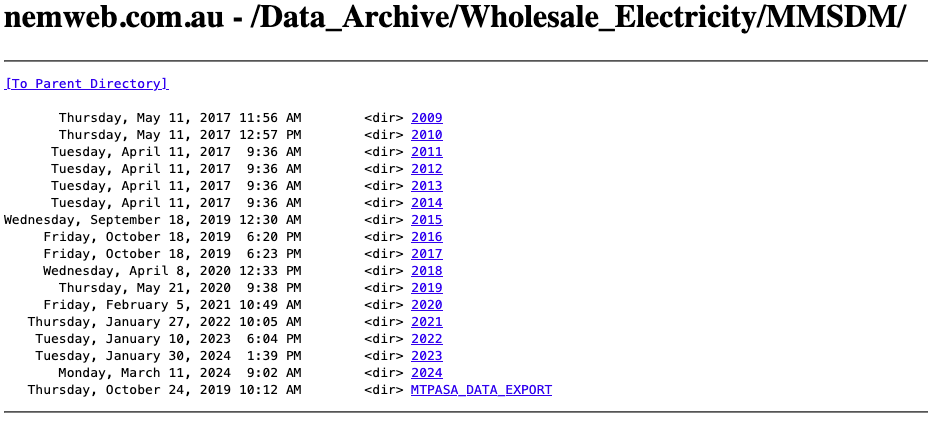
\includegraphics{img/nemweb-1.png}
\caption{Data\_Archive/Wholesale\_Electricity/MMSDM}
\end{figure}

And when we access a year, we get a more granular view of the months.:

\begin{figure}
\centering
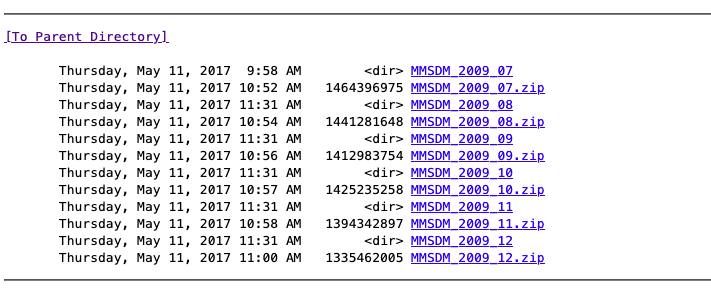
\includegraphics{img/nemweb-2.png}
\caption{Data\_Archive/Wholesale\_Electricity/MMSDM}
\end{figure}

=======

\begin{quote}
\begin{quote}
\begin{quote}
\begin{quote}
\begin{quote}
\begin{quote}
\begin{quote}
4fd6061ac55237b464961a42b9359505323e5e0c For the puposes of this
project, we are interested in the data between 2017 and 2023
\end{quote}
\end{quote}
\end{quote}
\end{quote}
\end{quote}
\end{quote}
\end{quote}

\subsubsection{Python code to download}\label{python-code-to-download}

For the project, Python's \texttt{requests} library was used to automate
the retrieval of ZIP files containing the data from the web. The URLs
were constructed dynamically for each month of each year within the
specified range, adhering to the naming convention and directory
structure observed on the website. The file names were prefixed and
suffixed appropriately to match the naming format provided by the site.

A \texttt{download\_file(url,\ path)} function was defined to manage the
HTTP request for each file's URL. If the server responded positively,
the content was written to a local file in a pre-determined directory,
ensuring the preservation of the data structure. This function printed
out the status of each download attempt, helping track progress and
identify any issues. The main block of the code iterated over each year
and month, constructed the full URL for the corresponding data file, and
called the \texttt{download\_file} function to perform the download.

The \texttt{Path} object from the \texttt{pathlib} library specified the
directory for storing the downloaded files and ensured that the
necessary directories existed. The code was initiated with a loop over
the specified range of years and months, systematically downloading each
file to the local system, thereby automating the process of data
collection for analysis or further processing. The completion of all
downloads was confirmed with a final print statement.

\subsubsection{Unzipping}\label{unzipping}

A further step leading to the loading of the data into a pandas
dataframe for analysis involved unzipping the files and storing them
into an organized folder structure. The Python \texttt{zipfile} library
was used to manage the extraction of ZIP files, while the
\texttt{pathlib} library took care of file path operations. The code
specified a directory containing the ZIP files and created a target
directory for the unzipped data, ensuring it existed before proceeding
with unzipping. A loop was implemented to iterate over each ZIP file
found in the specified directory. For each file, the
\texttt{zipfile.ZipFile(file,\textquotesingle{}r\textquotesingle{})}
method was invoked to open the ZIP file in read mode, and contents were
extracted into the designated unzipped directory. Each successful
extraction was acknowledged with a print statement indicating the file's
name and the destination of the unzipped content.

\subsubsection{\texorpdfstring{Loading Into \texttt{pandas}
Dataframes}{Loading Into pandas Dataframes}}\label{loading-into-pandas-dataframes}

Now that the unzipped files were in place, it was time to load them, and
pandas was used for this purpose. The Python script utilized the
\texttt{pathlib} and \texttt{pandas} libraries to facilitate file
management and data manipulation. Initially, the script identified all
CSV files in the designated directory, storing the paths to these files
in a list. If no CSV files were found, the script printed a notification
message.

Once the file paths were established, the script loaded the first CSV
file to establish a baseline for the column structure using pandas'
\texttt{read\_csv} function with the \texttt{header=1} parameter, which
specified that the second row of the file should be treated as the
header. The columns from this initial file were stored and printed.

The script then iterated over the remaining CSV files in the list,
loading each one to compare its column structure against the baseline.
If a file's column structure did not match the baseline, a flag was set
to false, and a message was printed indicating which file differed.
Finally, the script checked the flag to determine if all files had a
consistent column structure, and appropriate messages were printed based
on this check. This process ensured that all data files were compatible
in terms of their structure before any further data processing or
analysis was performed.

\subsubsection{Combining into one
Dataframe}\label{combining-into-one-dataframe}

Our final step before analysis was to have a combined CSV. Using
Python's \texttt{pandas} library and the \texttt{pathlib} module, the
script performed this integration. First, it searched through the
specified directory to find all CSV files, reading each one into a
separate DataFrame. The \texttt{header=1} parameter was used to ensure
the second row of each file was used as the header.

After all individual DataFrames were created and stored in a list, the
script combined them into a single DataFrame using
\texttt{pandas.concat}, with the \texttt{ignore\_index=True} option to
reset the index in the resulting DataFrame. This approach ensured that
the data from each file was seamlessly appended without any index
overlap.

The combined DataFrame was then saved back to disk as a new CSV file in
the same directory as the original files, ensuring all data was
consolidated in one accessible location. The path for the new combined
CSV was constructed using the \texttt{pathlib} module to maintain
consistency with file handling operations. The completion of this task
was confirmed with a print statement that indicated the location of the
saved combined CSV file, marking the readiness of the data for
subsequent analysis steps.

\section{Describing the Data}\label{describing-the-data}

\subsection{Description of the Github
Data}\label{description-of-the-github-data}

\textbf{General Overview The Github Data}

The given data that the team will be examining is stored as CSV files in
Github. It includes independent variables such as the date of the year,
the location and recorded temperature; and dependent variables such as
the total demand and the forecasted demand. In total, we are dealing
with 13 million, which can be considered as a large dataset. The data is
a time series which can introduce more complexity in the model. This
complexity, together with the size of the data are uan indicator that
the usage of GPUs to accelerate the training of our model. Tools such as
Google Colab Pro provide this service.

\textbf{Dataset: totaldemand\_nsw.csv, totaldemand\_vic.csv,
totaldemand\_qld.csv, totaldemand\_sa.csv, totaldemand\_tas.csv1}

This dataset contains the total energy demand around Australia from 2010
to March 2021. The demand listed in the dataset will be used to predict
the demand in the next 1 to 5 years and how solar panels affects the
total demand. There are shortcoming on this dataset as the data included
in the 2021 is only up to March, hence for the purpose of our research,
the year of 2021 will be omitted.

\textbf{Dataset: temperature\_nsw.csv, temperature\_vic.csv,
temperature\_qld.csv, temperature\_tas.csv, temperature\_sa.csv2}

This dataset records the temperature data from across Australia from
2010 to March 2021. Do note that this set of data only records the
temperature from one location in the state. The temperature listed in
the dataset will be used to predict the demand in the next 1 to 5 years
and how solar panels affects the total demand. Again, this dataset has
the same shortcomings with the previous dataset as the data included in
the 2021 is only up to March, hence for the purpose of our research, the
year of 2021 will be omitted as well. Another shortcoming is that the
temperatures recorded in QLD and in SA are identical. This might be due
to a an error with data storage and loading.

\textbf{Dataset: combined\_df\_grouped\_sorted.csv}

The dataset contains the rooftop Photovoltaic (PV) output from the state
of Queensland, New South Wales, Tasmania, and Victoria from 2017 to
2022. It was made up with monthly PV outdata data downloaded from AEMO
and combined using python. Please note that this dataset only records
the output in one location of each state. The dataset records the PV
output in 30-minute intervals. This dataset will be used for predicting
the energy demand along with using temperature data listed from above.
This dataset was sourced from AEMO on their website. The csv file is
around 12.2MB and contains around 420,000 lines of data.

\textbf{Dataset: Aus\_public\_hols\_2009-2022-1.csv}

The dataset contains public holiday of each state in Australia from 2009
to 2022. Since the demand during weekends and publics holidays are
usually higher than a working day, by implementing the public holidays
to the model will help improves its accuracy. The size of the file is
around 41KB and contains around 650 lines of data. This dataset is also
stored on Github for easy access.

\subsection{Description of Scraped Rooftop PV
Data}\label{description-of-scraped-rooftop-pv-data}

\textbf{Description of the rooftop PV data}

\_Todo\_\_ \#\# Pre-processing Steps

The key steps we followed to prepare the data for processing can be
broadly grouped into eight sections as follows

\textbf{1. Unzip the files and import the data}

The data scraping and unzipping procedures are described in detail
above, including obtaining the additional PV data. Once the data was
downloaded, unzipped, and ready, it was then converted into dataframes
using the code below.

\begin{Shaded}
\begin{Highlighting}[]
\NormalTok{temperature\_vic }\OperatorTok{=}\NormalTok{ pd.read\_csv(}\StringTok{"../Data/temperature\_vic.csv"}\NormalTok{)}
\NormalTok{temperature\_qld }\OperatorTok{=}\NormalTok{ pd.read\_csv(}\StringTok{"../Data/temperature\_qld.csv"}\NormalTok{)}
\OperatorTok{\textless{}\textless{}\textless{}\textless{}\textless{}\textless{}\textless{}}\NormalTok{ HEAD}
\NormalTok{temperature\_sa }\OperatorTok{=}\NormalTok{ pd.read\_csv(}\StringTok{"C:../Data/temperature\_sa.csv"}\NormalTok{)}
\OperatorTok{=======}
\NormalTok{temperature\_sa }\OperatorTok{=}\NormalTok{ pd.read\_csv(}\StringTok{"../Data/temperature\_sa.csv"}\NormalTok{)}
\OperatorTok{\textgreater{}\textgreater{}\textgreater{}\textgreater{}\textgreater{}\textgreater{}\textgreater{}} \DecValTok{4}\ErrorTok{fd6061ac55237b464961a42b9359505323e5e0c}
\NormalTok{forecastdemand\_vic }\OperatorTok{=}\NormalTok{ pd.read\_csv(}\StringTok{"../Data/forecastdemand\_vic.csv"}\NormalTok{)}
\NormalTok{forecastdemand\_qld }\OperatorTok{=}\NormalTok{ pd.read\_csv(}\StringTok{"../Data/forecastdemand\_qld.csv"}\NormalTok{)}
\NormalTok{forecastdemand\_sa }\OperatorTok{=}\NormalTok{ pd.read\_csv(}\StringTok{"../Data/forecastdemand\_sa.csv"}\NormalTok{)}
\NormalTok{totaldemand\_vic }\OperatorTok{=}\NormalTok{ pd.read\_csv(}\StringTok{"../Data/totaldemand\_vic.csv"}\NormalTok{)}
\NormalTok{totaldemand\_qld }\OperatorTok{=}\NormalTok{ pd.read\_csv(}\StringTok{"../Data/totaldemand\_qld.csv"}\NormalTok{)}
\NormalTok{totaldemand\_sa }\OperatorTok{=}\NormalTok{ pd.read\_csv(}\StringTok{"../Data/totaldemand\_sa.csv"}\NormalTok{)}
\end{Highlighting}
\end{Shaded}

\textbf{2. Check what sort of data is contained} This was achieved by
running the following python queries across each of the dataframes
(approach used for South Australian datasets shown below):

\#Temperature SA:

\begin{Shaded}
\begin{Highlighting}[]
\CommentTok{\# Column names}
\BuiltInTok{print}\NormalTok{(}\StringTok{"Column names for temperature\_sa:"}\NormalTok{)}
\BuiltInTok{print}\NormalTok{(temperature\_sa.columns.tolist())}

\CommentTok{\# Data types}
\BuiltInTok{print}\NormalTok{(}\StringTok{"}\CharTok{\textbackslash{}n}\StringTok{Data types for temperature\_sa:"}\NormalTok{)}
\BuiltInTok{print}\NormalTok{(temperature\_sa.dtypes)}

\CommentTok{\# Summary statistics}
\BuiltInTok{print}\NormalTok{(}\StringTok{"}\CharTok{\textbackslash{}n}\StringTok{Summary statistics for temperature\_sa:"}\NormalTok{)}
\BuiltInTok{print}\NormalTok{(temperature\_sa.describe())}
\end{Highlighting}
\end{Shaded}

This exploration showed that a `DATETIME' column existed in each
dataset, but was formatted as object type, rather than data time.
Further exploration showed that not all the DATETIME fields were in the
same format.

\textbf{3. Convert DATETIME to correct format}

The DATETIME fields for each of the datasets were reviewed, and they
could be automatically converted using Python's built-in
`pd.to\_datetime' function. However, in the case of `temperature\_qld',
the format was different and required manual intervention, as shown in
the code below, to ensure it converted correctly.

\begin{Shaded}
\begin{Highlighting}[]
\NormalTok{temperature\_qld[}\StringTok{\textquotesingle{}DATETIME\textquotesingle{}}\NormalTok{] }\OperatorTok{=}\NormalTok{ pd.to\_datetime(temperature\_qld[}\StringTok{\textquotesingle{}DATETIME\textquotesingle{}}\NormalTok{], }\BuiltInTok{format}\OperatorTok{=}\StringTok{\textquotesingle{}}\SpecialCharTok{\%d}\StringTok{/\%m/\%Y \%H:\%M\textquotesingle{}}\NormalTok{) }
\CommentTok{\# This date format is different}
\end{Highlighting}
\end{Shaded}

\textbf{4. Check for duplicate data records}

Duplicates were checked for each of the regional datasets by applying
the `.duplicated' function from the Pandas library in Python,
specifically to the `DATETIME' column. Duplicate values were expected to
exist in other columns.

An example of the code used to check and count duplicates is as follows:

\begin{Shaded}
\begin{Highlighting}[]
\NormalTok{duplicate\_count\_demand\_vic }\OperatorTok{=}\NormalTok{ forecastdemand\_vic.duplicated(}\StringTok{\textquotesingle{}DATETIME\textquotesingle{}}\NormalTok{).}\BuiltInTok{sum}\NormalTok{()}
\end{Highlighting}
\end{Shaded}

Plotting the results quickly revealed a significant number of duplicates
in the forecast demand dataframe, labeled `demand\_' in the plots below.

\subsubsection{Victoria}\label{victoria}

\begin{figure}
\centering
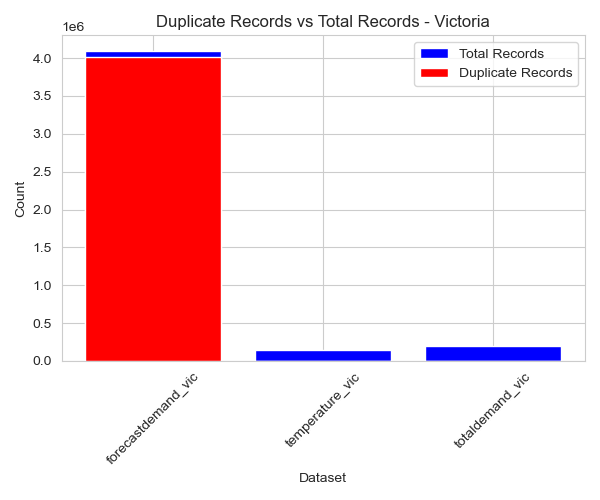
\includegraphics{img/duplicate_check_vic.png}
\caption{Duplicate check VIC:}
\end{figure}

\subsubsection{South Australia}\label{south-australia}

\begin{figure}
\centering
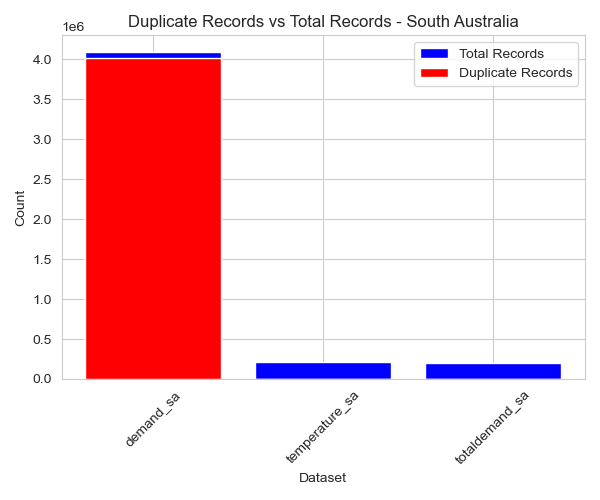
\includegraphics{img/duplicate_check_SA.png}
\caption{Duplicate check SA:}
\end{figure}

\subsubsection{Queensland}\label{queensland}

\begin{figure}
\centering
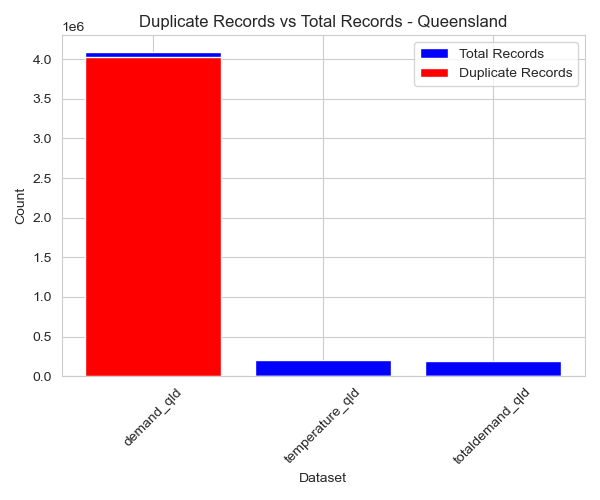
\includegraphics{img/duplicate_check_QLD.png}
\caption{Duplicate check QLD:}
\end{figure}

After examining these charts, it was unclear what caused the duplicates.
To investigate further, the original CSV files were inspected in a text
editor. It was discovered that the source of the duplicates stemmed from
updates to the forecast demand files, which periodically provided new
demand estimates for the same forecast time horizon. These updated
estimates offered a refreshed set of demand forecasts for the same
period.

Upon counting these duplicates, it was found that there were 73,836
unique values for estimating the Forecast Demand, with an average time
interval between each estimate of approximately 30 minutes. This
suggests that a computer model re-estimated forecast demand every 30
minutes, generating a new estimate for the value of Forecast Demand for
that period.

Given the data types and context, duplicates of other field values were
expected, so no duplicate checking was performed on these fields.

\textbf{5. Drop Duplicates}

To drop the duplicates, we decided as a team to select the most recent
estimate of `FORECASTDEMAND' and exclude all prior estimates from the
dataframe. The following code was used:

\begin{Shaded}
\begin{Highlighting}[]
\NormalTok{forecastdemand\_qld\_no\_duplicates }\OperatorTok{=}\NormalTok{ forecastdemand\_qld.drop\_duplicates}
\NormalTok{(subset}\OperatorTok{=}\StringTok{\textquotesingle{}DATETIME\textquotesingle{}}\NormalTok{, keep}\OperatorTok{=}\StringTok{\textquotesingle{}last\textquotesingle{}}\NormalTok{)}
\end{Highlighting}
\end{Shaded}

Removing all duplicates facilitated the merging of the tables based on
the DATETIME field. Consequently, the count of FORECASTDEMAND values for
each of the three states (VIC, QLD, and SA) is now equal at 73,833.

\begin{Shaded}
\begin{Highlighting}[]
\NormalTok{forecastdemand\_qld.describe()}
\end{Highlighting}
\end{Shaded}

\textbf{6. Merge Dataframes by Region}

\subsubsection{Inspect Time Horizons}\label{inspect-time-horizons}

Prior to merging on the DATETIME field, further exploration of the time
horizons covered by each data sets was conducted with the results shown
below.

\begin{figure}
\centering
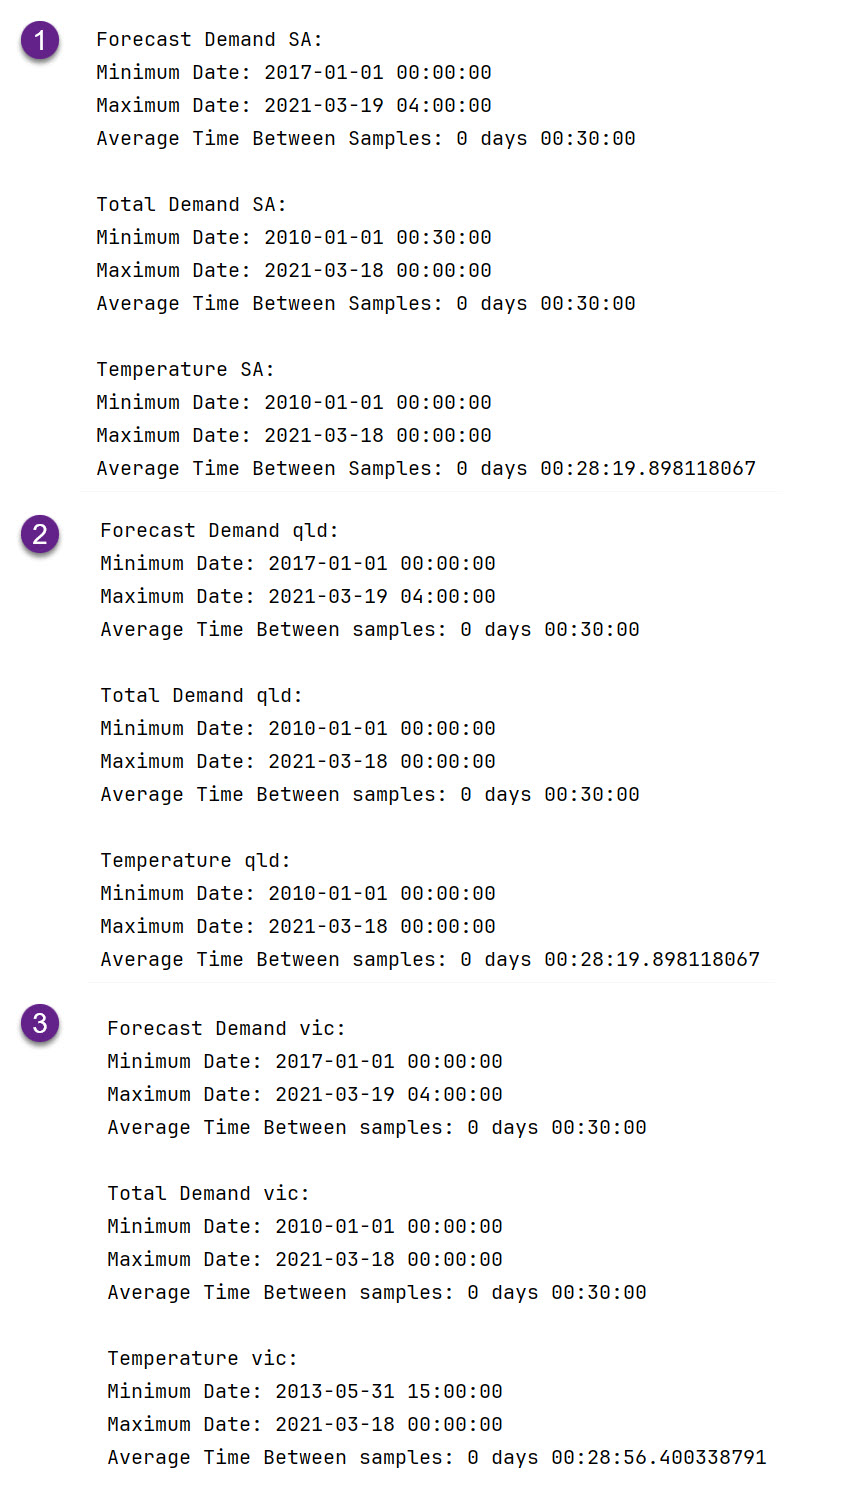
\includegraphics{img/DataFrameTimeHorizons.jpg}
\caption{Data Frame Time Horizon Check:}
\end{figure}

The analysis reveals that for each region, Forecast Demand typically
spans from January 1, 2017, to March 19, 2021, covering a period of a
bit over 4 years. In comparison, the temperature and demand data
typically cover a longer period, from January 1, 2010, to March 19,
2021, totaling a bit more than 11 years.

Merging the datasets based on DATETIME naturally reduces the dataset to
the smallest data range common to all three datasets. This excludes
approximately 7 years of data, from January 2010 to January 2017.

Considering the size of the remaining dataset, which consists of
30-minute data over more than 4 years, it was deemed more than
sufficient for training a model, especially given the computational
advantages with the smaller dataset. Additionally, collecting PV data
dating back to 2010 presented further challenges.

\subsubsection{Merge into QLD, SA and VIC
dataframes}\label{merge-into-qld-sa-and-vic-dataframes}

The 3 individual dataframes for each region were then merged into a
single combined dataframe for each region. 1) temperature\_qld 2)
totaldemand\_qld 3) forecastdemand\_qld

The below code was used to complete a two step `inner join' to create a
single file.

\begin{Shaded}
\begin{Highlighting}[]
\NormalTok{qld\_df }\OperatorTok{=}\NormalTok{ pd.merge(temperature\_qld, totaldemand\_qld, on}\OperatorTok{=}\StringTok{\textquotesingle{}DATETIME\textquotesingle{}}\NormalTok{, how}\OperatorTok{=}\StringTok{\textquotesingle{}inner\textquotesingle{}}\NormalTok{)}
\NormalTok{qld\_df }\OperatorTok{=}\NormalTok{ pd.merge(qld\_df, forecastdemand\_qld, on}\OperatorTok{=}\StringTok{\textquotesingle{}DATETIME\textquotesingle{}}\NormalTok{, how}\OperatorTok{=}\StringTok{\textquotesingle{}inner\textquotesingle{}}\NormalTok{)}
\end{Highlighting}
\end{Shaded}

\textbf{7. Handling Missing Values} Missing values were routinely
checked in all dataframes during import and initial inspection. After
merging the dataframes, a final check for missing values was conducted
in each of the three dataframes using the following Python command. This
revealed that there were no missing values in any of the dataframes.

\begin{Shaded}
\begin{Highlighting}[]
\NormalTok{total\_missing\_sa }\OperatorTok{=}\NormalTok{ sa\_df.isnull().}\BuiltInTok{sum}\NormalTok{().}\BuiltInTok{sum}\NormalTok{()}
\BuiltInTok{print}\NormalTok{(}\StringTok{"Total missing values SA:"}\NormalTok{, total\_missing\_sa)}
\end{Highlighting}
\end{Shaded}

\textbf{8. Checking for outliers}

Boxplots were generated for the key fields of interest, including
`TEMPERATURE', `TOTALDEMAND', and `FORECASTDEMAND'. Upon observing these
plots (for QLD), it is evident that the temperature range falls within
expected values, ranging from a little above zero to slightly above 40
degrees Celsius. Additionally, `TOTALDEMAND' and `FORECASTDEMAND'
exhibit similar patterns, as expected, and there are no outliers beyond
what would normally be expected.

\begin{figure}
\centering
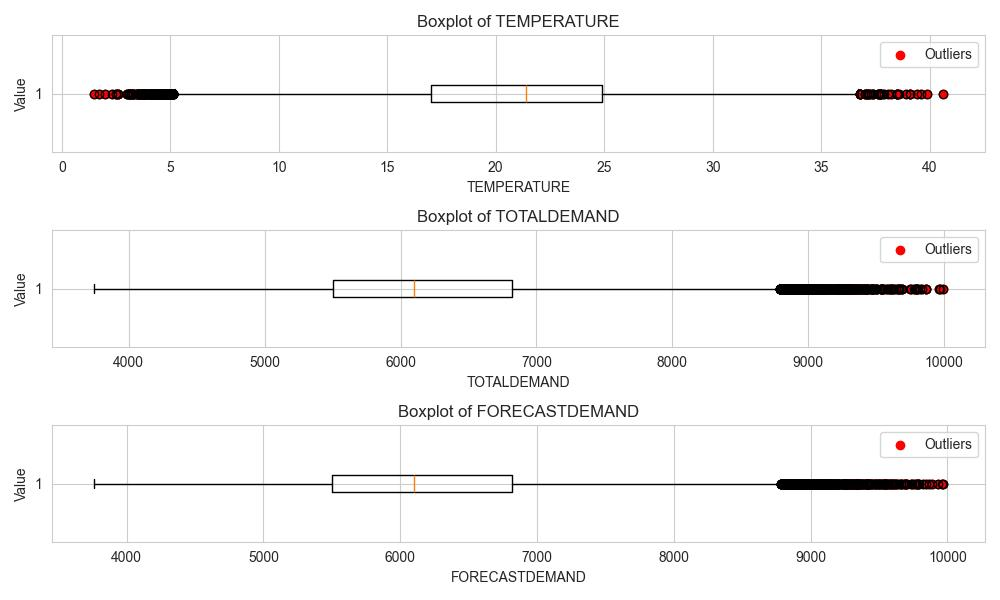
\includegraphics{img/OutlierBoxPlots.jpg}
\caption{QLD Outlier Box Plots:}
\end{figure}

Histograms for the same fields further support this outlier analysis.

\begin{figure}
\centering
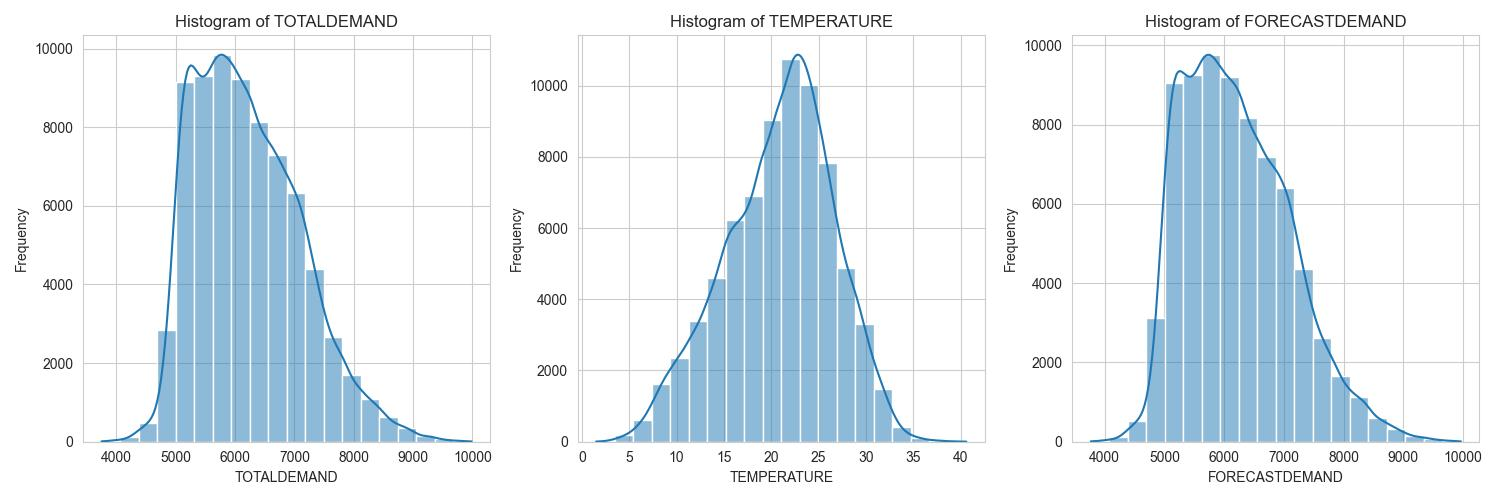
\includegraphics{img/Histogram.jpg}
\caption{QLD Histograms:}
\end{figure}

\subsection{Assumptions}\label{assumptions}

The assumprions made on the data is that it is accurate and reliable.
This is in addition to the assumptions about data type discussion in the
previous sections.

\section{Modelling}\label{modelling}

\subsection{Introduction to Modelling
Methods}\label{introduction-to-modelling-methods}

In this section, we present the modelling methods employed to forecast
the total electricity demand in the NEM. Given the complexity of the
factors influencing electricity consumption, multiple modelling
approaches have been utilised to capture various patterns and
dependencies in the data.

To address the challenge of forecasting electricity demand, we have
deployed several statistical and machine learning models, each offering
unique strengths and suited to capturing different aspects of the data.
The models selected for this study include:

\begin{enumerate}
\def\labelenumi{\arabic{enumi}.}
\tightlist
\item
  Linear Regression Model: This model leverages historical demand data
  to capture linear trends and seasonal variations, providing a baseline
  for performance comparison.
\item
  Neural Network Model (MLP): A Multi-Layer Perceptron (MLP), a type of
  neural network, is used to model non-linear relationships in the data.
  Its ability to learn complex patterns makes it suitable for the
  non-linear dynamics of electricity demand.
\item
  Stacked Model: Combining Generalised Boosted Models (GBM), Linear
  Regression, and MLP, this ensemble approach leverages the strengths of
  individual models to improve overall prediction accuracy. The stacking
  method helps in reducing the variance and bias of the forecast,
  capitalising on the diverse predictive capabilities of the constituent
  models.
\item
  Long Short-Term Memory (LSTM) Model: An LSTM model is specifically
  designed to address time-series data like electricity demand, which
  requires understanding long-term dependencies in data due to factors
  such as seasonal effects and economic cycles.
\end{enumerate}

Each model has been chosen based on its potential to effectively handle
the characteristics of the dataset and the specific forecasting
requirements of the electricity market. The subsequent sections will
detail the configuration, feature engineering, and performance
evaluation of each model, providing insights into their comparative
effectiveness and the rationale behind the final model selection.

\subsection{Description of Each Model}\label{description-of-each-model}

\textbf{1. Basic Linear Regression Model}

Model Overview: Linear regression is a foundational statistical method
used for modeling the relationship between a dependent variable and one
or more independent variables by fitting a linear equation to observed
data. The equation for a linear regression line is typically in the
form:

The equation for a linear regression line is typically in the form:

\[ y = \beta_0 + \beta_1 x_1 + \dots + \beta_n x_n \]

where: - \(y\) is the predicted value, - \(\beta_0\) is the intercept, -
\(\beta_i\) are the coefficients for each feature, - \(x_i\) are the
feature values.

This model is well-suited for cases where the relationship between
variables is expected to be linear.

Rationale for Inclusion: The basic Linear Regression model is included
in this study due to its effectiveness in providing a clear and
straightforward understanding of the influences of different predictors
on electricity demand. It serves as a fundamental benchmark for
evaluating more complex models. The model's simplicity and
interpretability are particularly valuable for initial exploratory
analyses, where understanding the direct linear impact of individual
factors---such as temperature, time of day, and economic indicators---on
electricity demand is crucial.

\textbf{2. Neural Network Model (MLP)}

Model Overview: The Multi-Layer Perceptron (MLP) is a type of neural
network known for its capability to model complex, non-linear
relationships through its multiple layers and neurons. MLPs are widely
used in pattern recognition, forecasting, and classification tasks where
the relationships between variables are not easily discernible or are
highly non-linear (Nielsen, 2015).

The MLP model consists of multiple layers: an input layer, one or more
hidden layers, and an output layer. Each layer (l) performs a linear
transformation followed by a non-linear activation:

\[ z^{(l)} = W^{(l)}a^{(l-1)} + b^{(l)} \]
\[ a^{(l)} = \sigma(z^{(l)}) \]

Where: - \(a^{(0)}\) is the input vector, - \(W^{(l)}\) and \(b^{(l)}\)
are the weight matrix and bias vector for layer \(l\) respectively, -
\(z^{(l)}\) is the linear combination at layer \(l\), - \(a^{(l)}\) is
the activation after applying the non-linear function \(\sigma\) at
layer \(l\), - \(\sigma\) is the activation function, such as Sigmoid,
ReLU, or Tanh.

The output of the final layer \(a^{(L)}\) is used for prediction:
\[ \hat{y} = a^{(L)} \]

This is the forward propagation mechanism. Learning in MLPs involves
adjusting \(W^{(l)}\) and \(b^{(l)}\) through backpropagation to
minimize the loss function comparing \(\hat{y}\) and the actual target
outputs.

Rationale for Inclusion: The MLP model is included in this project to
leverage its ability to capture intricate patterns in the data that
simpler models might miss. The non-linear dynamics of electricity
demand, influenced by numerous factors such as economic activity,
unpredictable weather conditions, and changes in consumer behaviour,
make MLP a suitable choice.

\textbf{3. Stacked Model}

Model Overview: A stacked model is an ensemble technique that combines
the predictions from multiple individual models to produce a final
output. The stacking method involves training a meta-model to synthesise
the outputs of the base models into a single prediction, aiming to
reduce bias and variance. In this specific application, the stacked
model includes Generalised Boosted Models (GBM), Linear Regression, and
a Multi-Layer Perceptron (MLP). Each base model independently processes
the input data and makes predictions which are then used as inputs for
the meta-model (Wolpert, 1992).

For example, suppose we have \(n\) base models, where each model \(m_i\)
provides a prediction \(p_i\) for the same input data \(x\). The
predictions of these base models are then used as input features for the
meta-model.

The process can be summarized by the following equations:

\begin{enumerate}
\def\labelenumi{\arabic{enumi}.}
\item
  Each base model \(m_i\) predicts the output:
  \[ p_i = m_i(x) \quad \text{for} \ i = 1, 2, \ldots, n \]
\item
  The meta-model \(M\) takes these predictions as inputs and combines
  them to produce the final prediction \(\hat{y}\):
  \[ \hat{y} = M(p_1, p_2, \ldots, p_n) \]
\end{enumerate}

where: - \(x\) is the input data, - \(p_i\) is the prediction from the
\(i\)-th base model, - \(\hat{y}\) is the final output from the
meta-model.

The meta-model is trained to optimize the combination of base models'
outputs, effectively learning the best way to integrate different
predictive signals to minimise the overall prediction error.

Rationale for Inclusion: The rationale for including a stacked model in
this study is rooted in its ability to leverage the diverse strengths of
various models to improve overall forecasting accuracy. Each of the
selected base models --- GBM, Linear Regression, and MLP --- captures
different aspects and complexities of the electricity demand forecasting
problem:

GBM is adept at handling nonlinear relationships and interactions
between variables, making it valuable for complex, hierarchical data
structures. Linear Regression provides clear insights into the linear
relationships and is highly interpretable, which is useful for
understanding direct impacts and trends. MLP, with its deep learning
capabilities, is good at at identifying patterns and dependencies in
large datasets that might be non-linear or hidden. By stacking these
models, we aim to mitigate the individual weaknesses of each model and
enhance prediction stability. The meta-model, a simpler model like
linear regression, is trained on the predictions of the base models,
ensuring that the final predictions are not just a simple average but a
weighted combination that considers how each model performs in various
scenarios.

\textbf{4. Long Short-Term Memory (LSTM) Model}

Model Overview: Long Short-Term Memory (LSTM) models are a kind of
Recurrent Neural Network (RNN) particularly well-suited to classifying,
processing, and predicting time series data given time lags of unknown
duration between important events. Unlike standard feedforward neural
networks, LSTMs have feedback connections that allow them to process not
just individual data points, but entire sequences of data (Hochreiter
and Schmidhuber, 1997). This feature makes them ideal for tasks where
context from the input data is crucial, such as speech recognition,
language modeling, and, importantly, time-series forecasting like
electricity demand.

An LSTM model is composed of various gates that control the flow of
information. These gates include the forget gate, input gate, and output
gate, which work together to update and maintain the cell state across
time steps. The equations that govern the behavior of an LSTM unit are
as follows (Chung et al., 2014):

\begin{enumerate}
\def\labelenumi{\arabic{enumi}.}
\item
  \textbf{Forget Gate:}
  \[ f_t = \sigma(W_f \cdot [h_{t-1}, x_t] + b_f) \] This gate decides
  what information to discard from the cell state. It looks at
  \(h_{t-1}\) (the previous hidden state) and \(x_t\) (the current
  input), and applies a sigmoid function.
\item
  \textbf{Input Gate:}
  \[ i_t = \sigma(W_i \cdot [h_{t-1}, x_t] + b_i) \]
  \[ \tilde{C}_t = \tanh(W_C \cdot [h_{t-1}, x_t] + b_C) \] The input
  gate updates the cell state by first deciding which values to update
  (using \(i_t\)), and then creating a vector of new candidate values
  (\(\tilde{C}_t\)) that could be added to the state.
\item
  \textbf{Update Cell State:}
  \[ C_t = f_t * C_{t-1} + i_t * \tilde{C}_t \] The cell state \(C_t\)
  is updated by forgetting the old state as decided by \(f_t\) and
  adding new candidate values scaled by \(i_t\).
\item
  \textbf{Output Gate:}
  \[ o_t = \sigma(W_o \cdot [h_{t-1}, x_t] + b_o) \]
  \[ h_t = o_t * \tanh(C_t) \] The output gate decides what the next
  hidden state should be. The state \(C_t\) is passed through \(\tanh\),
  which is then scaled by \(o_t\) to decide the output \(h_t\).
\end{enumerate}

where: - \(x_t\) is the input vector at time step \(t\), - \(h_t\) is
the hidden state at time step \(t\), - \(C_t\) is the cell state at time
step \(t\), - \(W\) and \(b\) are the weights and biases for different
gates, - \(\sigma\) is the sigmoid activation function, - \(\tanh\) is
the hyperbolic tangent activation function.

These components work together to allow the LSTM to maintain a long-term
memory, making it particularly effective for time-series data where the
context from previous events is crucial for understanding the current
state.

Rationale for Inclusion: The decision to include an LSTM model in this
study stems from its proven capability in handling sequential data with
dependencies over time, which is a common characteristic of electricity
usage data (Yuansheng et al., 2016). Electricity demand forecasting
involves understanding patterns that unfold over time, influenced by
factors such as weather, time of day, and economic conditions.
Traditional models often struggle with capturing these temporal dynamics
effectively, especially when the sequences have long time dependencies.

LSTMs are designed to overcome the vanishing gradient problem that can
occur with standard RNNs in the training process, allowing them to learn
from data where important events are separated by long time lags. This
capability is critical for accurately predicting electricity demand
where previous consumption patterns and external factors like weather
conditions can significantly influence future demand.

\section{Feature Engineering}\label{feature-engineering}

Feature engineering was a fundamental step in the data preprocessing
pipeline that significantly enhanced model performance. By transforming
raw data into new features, our models signficantly improved performance
over the baseline.

\textbf{Engineered Features:}

\begin{enumerate}
\def\labelenumi{\arabic{enumi}.}
\tightlist
\item
  Cooling Degree Days (CDD) Feature:
\end{enumerate}

Description: The `Cooling' feature represents the Cooling Degree Days,
calculated as the number of degrees where the temperature is above a
certain threshold (24°C here), indicating the energy demand for cooling.

Justification: This feature is essential in Australia where air
conditioning is widely used. A temperature above 24°C would typically
result in increased electricity usage for cooling, making this a
relevant predictor for demand forecasting.

\begin{enumerate}
\def\labelenumi{\arabic{enumi}.}
\setcounter{enumi}{1}
\tightlist
\item
  Heating Degree Days (HDD) Feature:
\end{enumerate}

Description: The `Heating' feature represents the Heating Degree Days,
calculated as the number of degrees where the temperature is below a
certain threshold (20°C here), indicating the energy demand for heating.

Justification: Similar to CDD, HDD accounts for additional energy demand
for heating when the temperature drops below a comfortable threshold, a
key consideration for accurate demand prediction in cooler seasons.

\begin{enumerate}
\def\labelenumi{\arabic{enumi}.}
\setcounter{enumi}{2}
\tightlist
\item
  Weekend Indicator Feature:
\end{enumerate}

Description: The `is\_weekend' binary feature indicates whether a given
date falls on a weekend.

Justification: Electricity patterns often differ on weekends due to
changes in commercial activity and personal routines. Recognising
weekends can help the model adjust its forecasts accordingly.

\begin{enumerate}
\def\labelenumi{\arabic{enumi}.}
\setcounter{enumi}{3}
\tightlist
\item
  Seasonal Feature:
\end{enumerate}

Description: The `season' feature categorizes dates into seasons
(`Summer', `Autumn', `Winter', `Spring') based on the month.

Justification: Seasonal variations significantly affect energy
consumption due to weather-related changes in heating and cooling needs.
This categorization aligns with Australia's distinct seasons, which
correspond to varying energy usage profiles throughout the year.

\begin{enumerate}
\def\labelenumi{\arabic{enumi}.}
\setcounter{enumi}{4}
\tightlist
\item
  Public Holiday Feature:
\end{enumerate}

Description: A binary feature derived from the `public\_holidays'
dataset, indicating whether a date is a public holiday.

Justification: Public holidays usually mean a reduction in commercial
activity and can affect residential electricity consumption patterns.
Including this feature helps in predicting atypical demand associated
with holidays.

\section{Exploratory Data Analysis}\label{exploratory-data-analysis}

\textless\textless\textless\textless\textless\textless\textless{} HEAD
Starting with initial high level checks, a histogram of temperature data
for each of the three regions is provided below. It show intuitively
that QLD and South Australia are the hottest, followed by Victoria.
======= Beginning with initial high-level checks, histograms of
temperature data for each of the three regions are provided below. It is
evident from the histograms that Queensland and South Australia
experience higher temperatures compared to Victoria, with Queensland and
South Australia being the hottest regions, followed by Victoria.
\textgreater\textgreater\textgreater\textgreater\textgreater\textgreater\textgreater{}
4fd6061ac55237b464961a42b9359505323e5e0c

\begin{figure}
\centering
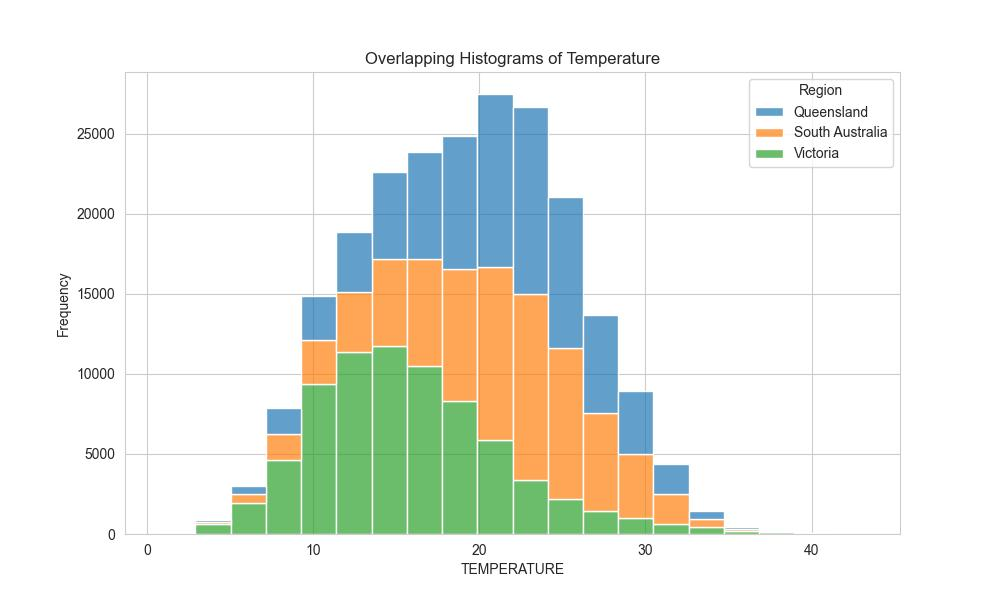
\includegraphics{img/Hist_Temperature.jpg}
\caption{Temperature Histogram:}
\end{figure}

A comparison of total demand by state is shown below:

\begin{figure}
\centering
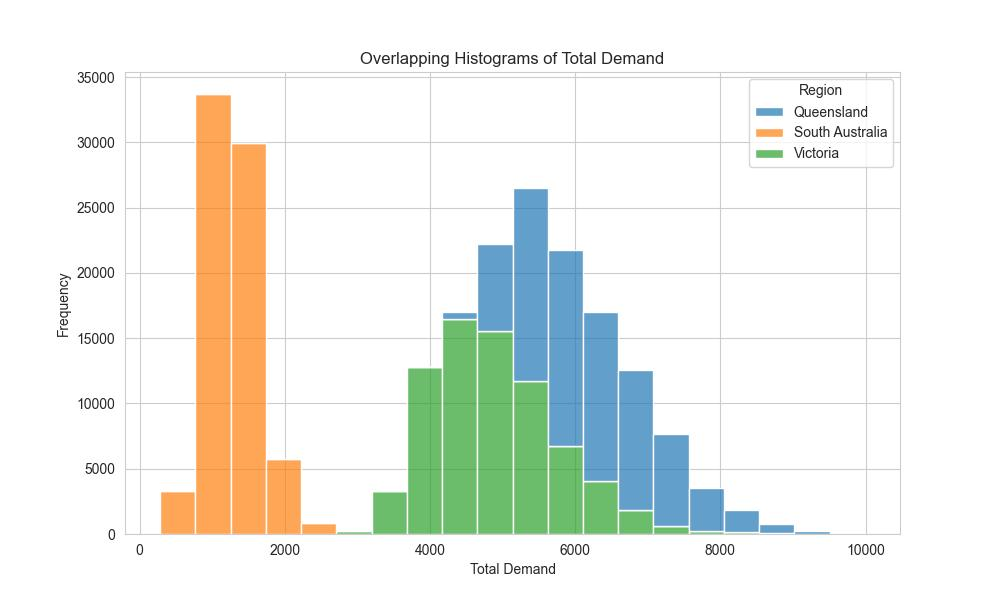
\includegraphics{img/Hist_TotalDemand.jpg}
\caption{Temperature Histogram:}
\end{figure}

\subsection{Relationship Between Time of Day and Power
Demand}\label{relationship-between-time-of-day-and-power-demand}

Examining the relationship between time of day and power demand reveals
interesting trends. Plotting the first 10 days of January 2010, we
observe a consistent correlation throughout the day for each region,
with demand typically peaking around midday and reaching its lowest
point in the early morning.

\begin{figure}
\centering
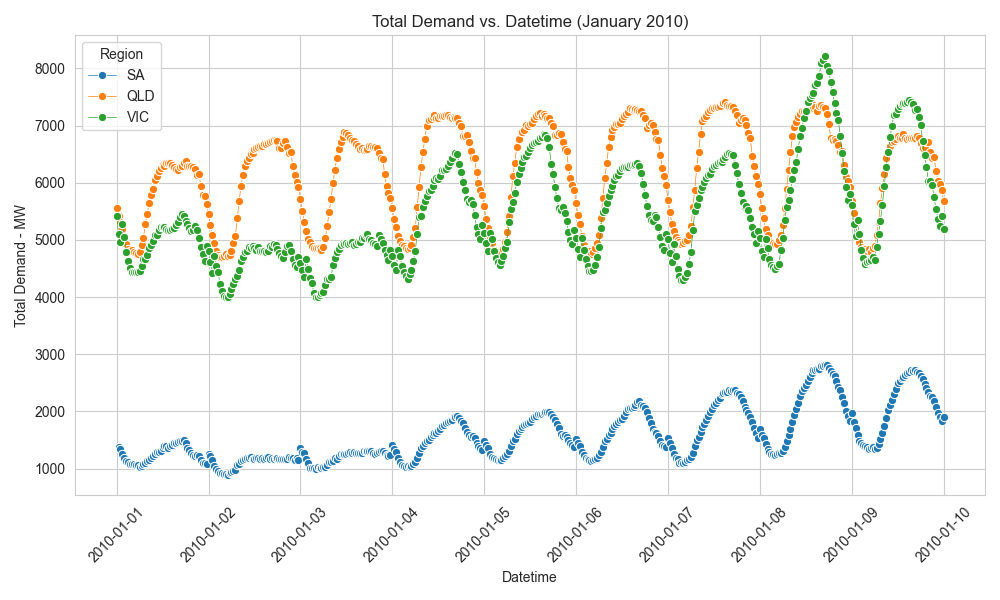
\includegraphics{img/TotalDemand_Jan2010.png}
\caption{Total Demand Comparison - 1st 10 days of Jan 2010:}
\end{figure}

\subsection{Relationship Between Temperature and
Demand}\label{relationship-between-temperature-and-demand}

We know from the literature review that temperature strongly influences
power demand. Filtering for different times of the day reveals this
relationship in XY scatter plots for 6 AM, noon, and 6 PM. It's evident
that the relationships at these times of day differ, as indicated by the
shape of the relationship.

\begin{figure}
\centering
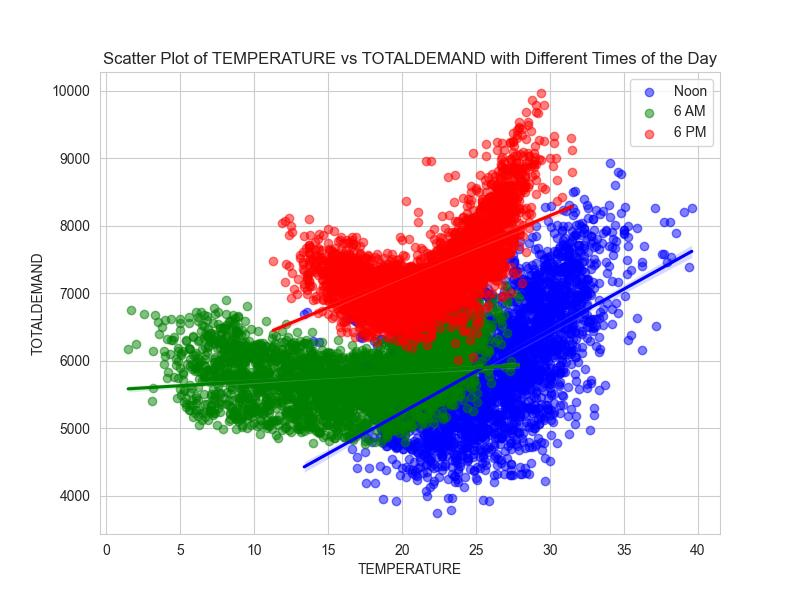
\includegraphics{img/Temp_vs_Demand_combined.jpg}
\caption{Temp\_vs\_Demand\_combined:}
\end{figure}

\textless\textless\textless\textless\textless\textless\textless{} HEAD
Exploring this further, and looking at 6pm for QLD we can see a strong
concave relationship (non linear) around a low point at close to 21
degrees.

Presumably as temperature moves further from this point, and the need
for air conditioning or heating increase, so too does power demand.

\begin{figure}
\centering
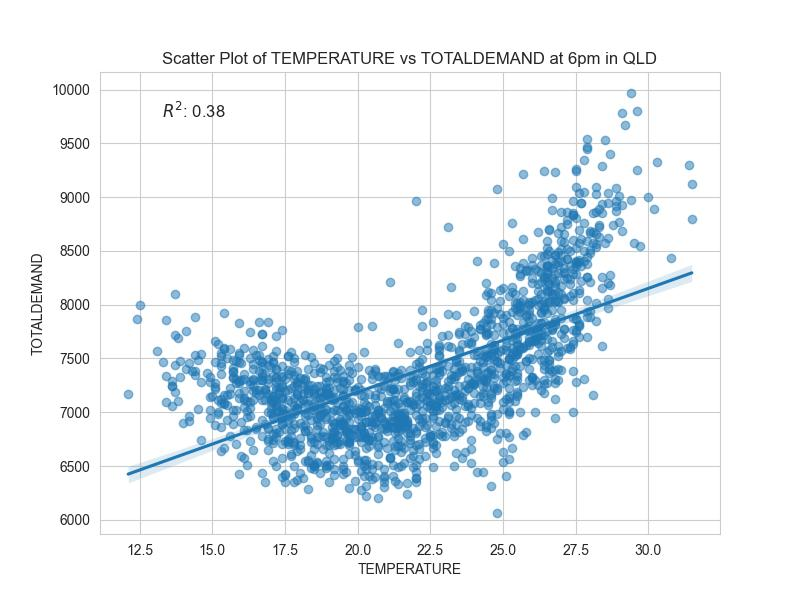
\includegraphics{img/Temp_vs_Demand_6pm.jpg}
\caption{Temp\_vs\_Demand\_6pm:}
\end{figure}

The relationship at midday is more linear in form, with average
temperatures close to 25 degrees, and therefore less of a requirement
for heating, and possibly less people at home turning on air
conditioners than in the evening.

\begin{figure}
\centering
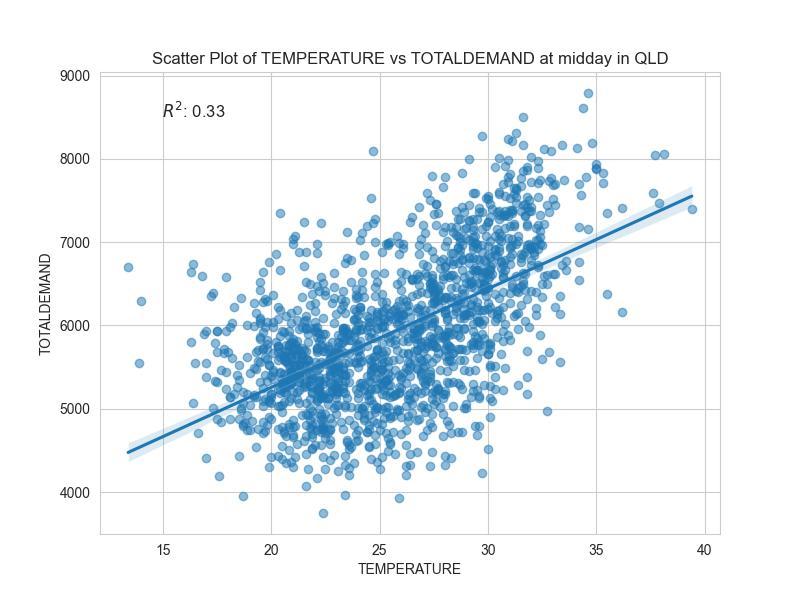
\includegraphics{img/Temp_vs_Demand_Noon.jpg}
\caption{Temp\_vs\_Demand\_Noon:}
\end{figure}

\section{looking at 6am, we can see a somewhat similar concave
relationship to 6pm, but with more variability. This
is}\label{looking-at-6am-we-can-see-a-somewhat-similar-concave-relationship-to-6pm-but-with-more-variability.-this-is}

Exploring this further, focusing on 6 PM for Queensland, we observe a
strong concave relationship around a low point at close to 21 degrees
Celsius. Presumably, as the temperature deviates from this point and the
need for air conditioning or heating increases, so does power demand.

\begin{figure}
\centering
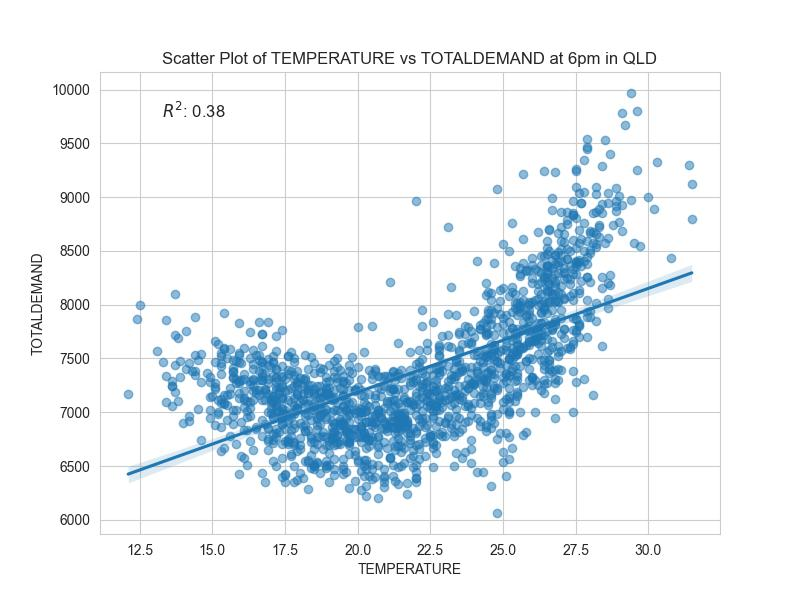
\includegraphics{img/Temp_vs_Demand_6pm.jpg}
\caption{Temp\_vs\_Demand\_6pm:}
\end{figure}

The relationship at midday is more linear in form, with average
temperatures close to 25 degrees Celsius. Consequently, there is less of
a requirement for heating, and possibly fewer people at home turning on
air conditioners than in the evening.

\begin{figure}
\centering
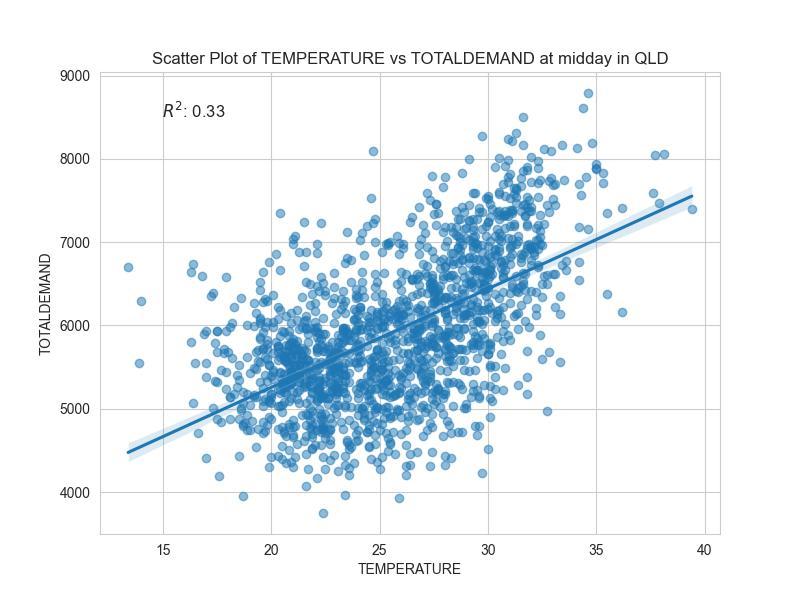
\includegraphics{img/Temp_vs_Demand_Noon.jpg}
\caption{Temp\_vs\_Demand\_Noon:}
\end{figure}

looking at 6am, we can see a somewhat similar concave relationship to
6pm, but with more variability.
\textgreater\textgreater\textgreater\textgreater\textgreater\textgreater\textgreater{}
4fd6061ac55237b464961a42b9359505323e5e0c

\begin{figure}
\centering
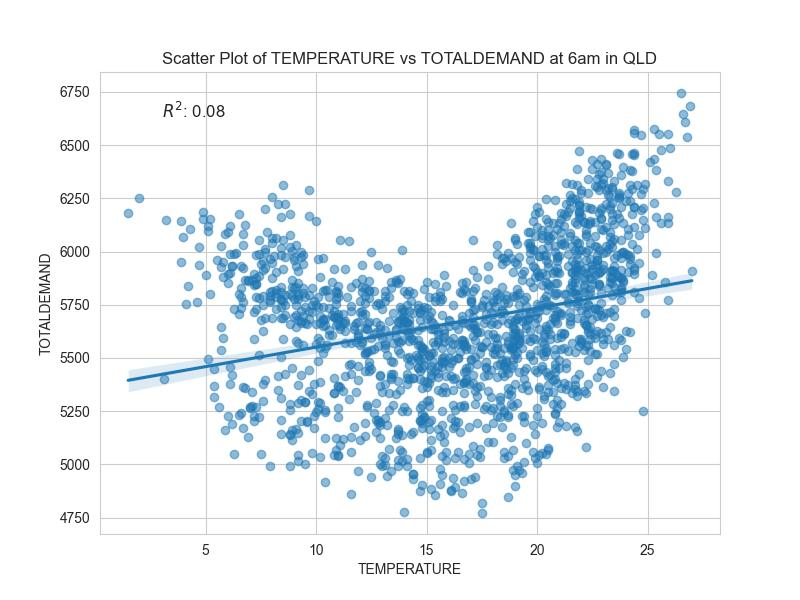
\includegraphics{img/Temp_vs_Demand_6am.jpg}
\caption{Temp\_vs\_Demand\_Noon:}
\end{figure}

\subsection{South Australia and
Victoria}\label{south-australia-and-victoria}

Looking at the Victoria data, we can see a stronger response to demand
as temperature decreases in the both the morning, but particularly the
evening.

\begin{figure}
\centering
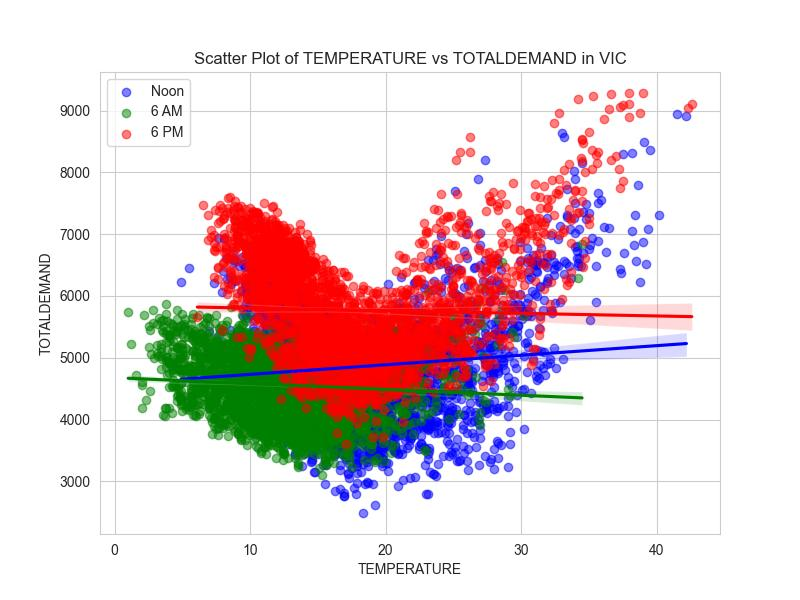
\includegraphics{img/Temp_vs_Demand_combined_VIC.jpg}
\caption{TTemp\_vs\_Demand\_combined\_VIC:}
\end{figure}

\textless\textless\textless\textless\textless\textless\textless{} HEAD
In South Australia, the trends are much less obvious, with demand
generally higher in the evening, but with this trend much less driven by
temperature. ======= In South Australia, the trends are much less
obvious, with demand generally higher in the evening. However, unlike in
other regions, this trend is less driven by temperature.
\textgreater\textgreater\textgreater\textgreater\textgreater\textgreater\textgreater{}
4fd6061ac55237b464961a42b9359505323e5e0c

\begin{figure}
\centering
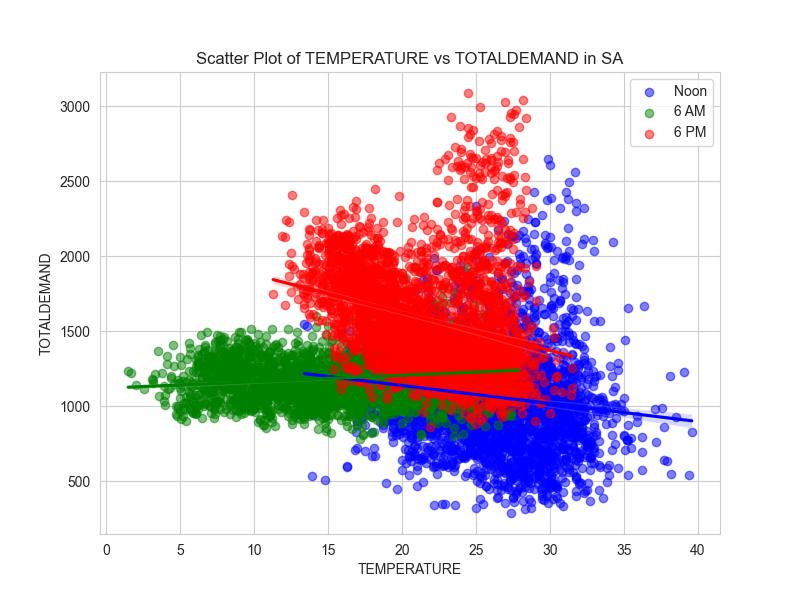
\includegraphics{img/Temp_vs_Demand_combined_SA.jpg}
\caption{TTemp\_vs\_Demand\_combined\_SA:}
\end{figure}

\section{Analysis and Results}\label{analysis-and-results}

In our analysis, we focused on modeling the Queensland dataset to
forecast electricity demand, based on the hypothesis that temperature
data alone may be a sufficient predictor. This hypothesis was
articulated as the null hypothesis:

\begin{itemize}
\tightlist
\item
  \textbf{Null Hypothesis} \$( H\_0 )\$: Temperature data alone is
  sufficient to reliably forecast electricity demand.
\end{itemize}

Our alternative hypothesis considered the inclusion of additional
features:

\begin{itemize}
\tightlist
\item
  \textbf{Alternative Hypothesis} \$( H\_1 )\$: Including the additional
  features of `solar generation capacity' and/or `solar radiation'
  improves the estimate of electricity demand.
\end{itemize}

The study centered on the Queensland dataset as a proof of concept, with
the intention to later replicate the methodology across other states.
The performance of various models was evaluated, spanning from Linear
Regression to more sophisticated approaches like MLP, LSTM, and Stacked
Models, with the comparison being drawn between models leveraging only
temperature data versus those incorporating engineered features.

The results, presented in the below tables, indicated a clear narrative:
models augmented with engineered features outperformed their simpler
counterparts across all metrics---MSE, RMSE, MAE, and \$ R\^{}2 \$. The
significant improvements in predictive accuracy and model fitness are
evidenced by lower error rates and higher \$ R\^{}2 \$ values.

Further analysis into the specific impact of solar features, as
reflected in the deltas shown in the second table, suggests a
substantial performance degradation when these features are excluded.
For instance, excluding solar features from the Linear Regression model
resulted in an MSE increase of over 103,000, underscoring the importance
of these predictors.

These findings provide a strong basis to reject the null hypothesis \$
H\_0 \$, and support the alternative hypothesis \$ H\_1 \$. The
integration of solar-related features has proven to be more than
marginally beneficial---it is a significant enhancement to the accuracy
of electricity demand forecasting. With the success of this proof of
concept in Queensland, our methodology is poised to be replicated across
other states, potentially increasing the precision of electricity demand
forecasts.

\begin{longtable}[]{@{}
  >{\raggedright\arraybackslash}p{(\columnwidth - 8\tabcolsep) * \real{0.6211}}
  >{\raggedright\arraybackslash}p{(\columnwidth - 8\tabcolsep) * \real{0.1263}}
  >{\raggedleft\arraybackslash}p{(\columnwidth - 8\tabcolsep) * \real{0.0842}}
  >{\raggedleft\arraybackslash}p{(\columnwidth - 8\tabcolsep) * \real{0.0842}}
  >{\raggedleft\arraybackslash}p{(\columnwidth - 8\tabcolsep) * \real{0.0842}}@{}}
\toprule\noalign{}
\begin{minipage}[b]{\linewidth}\raggedright
Model
\end{minipage} & \begin{minipage}[b]{\linewidth}\raggedright
MSE
\end{minipage} & \begin{minipage}[b]{\linewidth}\raggedleft
RMSE
\end{minipage} & \begin{minipage}[b]{\linewidth}\raggedleft
MAE
\end{minipage} & \begin{minipage}[b]{\linewidth}\raggedleft
R2
\end{minipage} \\
\midrule\noalign{}
\endhead
\bottomrule\noalign{}
\endlastfoot
Linear Regression & 649,170.19 & 805.71 & 657.72 & 0.1878 \\
Linear Regression with Engineered Features & 239,856.55 & 489.75 &
395.37 & 0.6947 \\
MLP with Engineered Features & 26,901.46 & 164.02 & 118.09 & 0.9658 \\
LSTM with Engineered Features & 20,508.91 & 143.21 & 103.19 & 0.9739 \\
Stacked Model with Engineered Features & 26,980.73 & 164.26 & 118.28 &
0.9657 \\
Linear Regression with Engineered Features - Except Solar & 342,977.48 &
585.64 & 466.78 & 0.5634 \\
MLP with Engineered Features - Except Solar & 45,649.33 & 213.66 &
152.13 & 0.9419 \\
LSTM with Engineered Features - Except Solar & 26,551.94 & 162.95 &
117.26 & 0.9662 \\
Stacked Model with Engineered Features - Except Solar & 45,511.44 &
213.33 & 151.54 & 0.9421 \\
\end{longtable}

Table 1: Raw Results of each Model with and without solar as a feature

\begin{longtable}[]{@{}llrrr@{}}
\toprule\noalign{}
Model & MSE & RMSE & MAE & R2 \\
\midrule\noalign{}
\endhead
\bottomrule\noalign{}
\endlastfoot
Linear Regression & -103,120.93 & -95.89 & -71.41 & 0.1313 \\
MLP & -18,747.87 & -49.64 & -34.03 & 0.0239 \\
LSTM & -6,043.03 & -19.74 & -14.07 & 0.0077 \\
Stacked Model & -18,530.71 & -49.08 & -33.26 & 0.0236 \\
\end{longtable}

Table 2: Delta between models with and without solar as a feature

Below, the first set of visualisations comprises a series of bar charts
that provide an overview of the performance of various predictive
models. Each chart represents a key metric used to evaluate the models,
such as Mean Squared Error (MSE), Root Mean Squared Error (RMSE), Mean
Absolute Error (MAE), and the coefficient of determination (\(R^2\)).
These models include the solar variable.

\begin{figure}
\centering
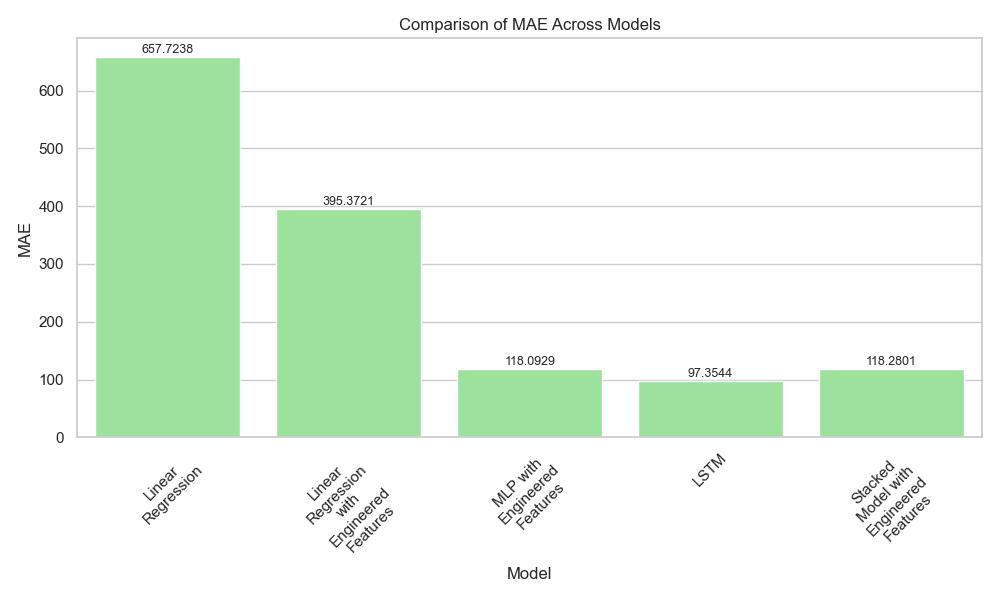
\includegraphics{img/mae_comparison_across_models.jpg}
\caption{MAE Across Models:}
\end{figure}

\begin{figure}
\centering
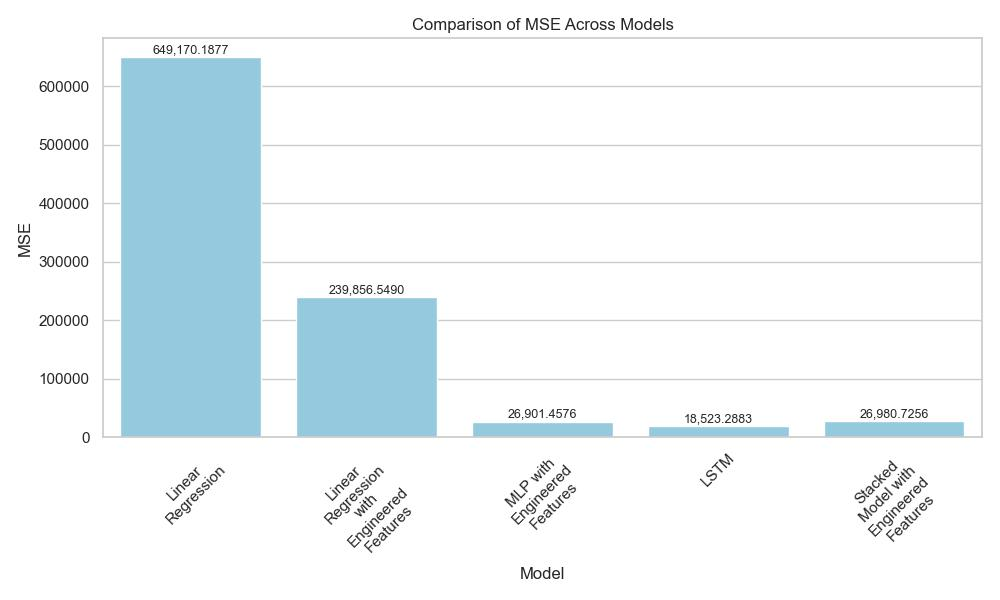
\includegraphics{img/mse_comparison_across_models.jpg}
\caption{MSE Across Models:}
\end{figure}

\begin{figure}
\centering
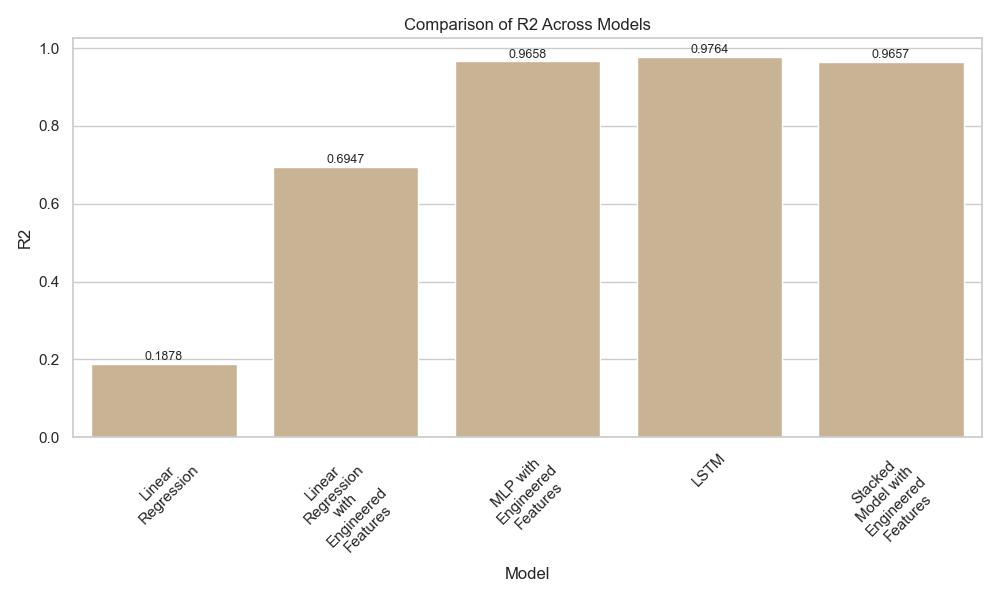
\includegraphics{img/r2_comparison_across_models.jpg}
\caption{R2 Across Models:}
\end{figure}

\begin{figure}
\centering
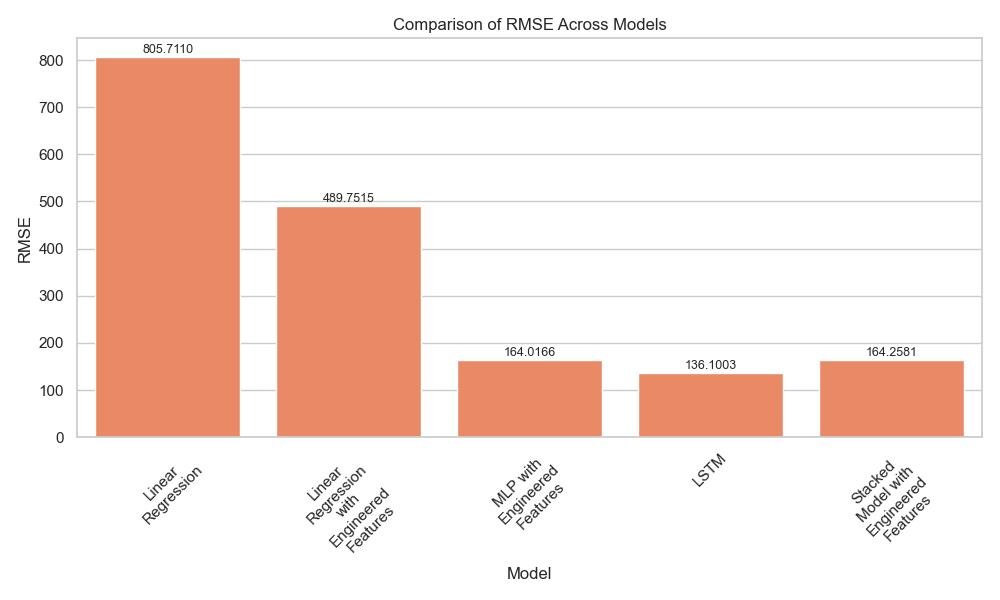
\includegraphics{img/rmse_comparison_across_models.jpg}
\caption{RMSE Across Models:}
\end{figure}

Following the histograms, the analysis transitions to a series of line
plots, tracing the performance of each individual model against the
actual recorded electricity demand. The temporal snapshot chosen for
this comparison is a randomly selected week in June---a period likely to
exhibit significant variation in electricity usage patterns due to
seasonal factors.

\begin{figure}
\centering
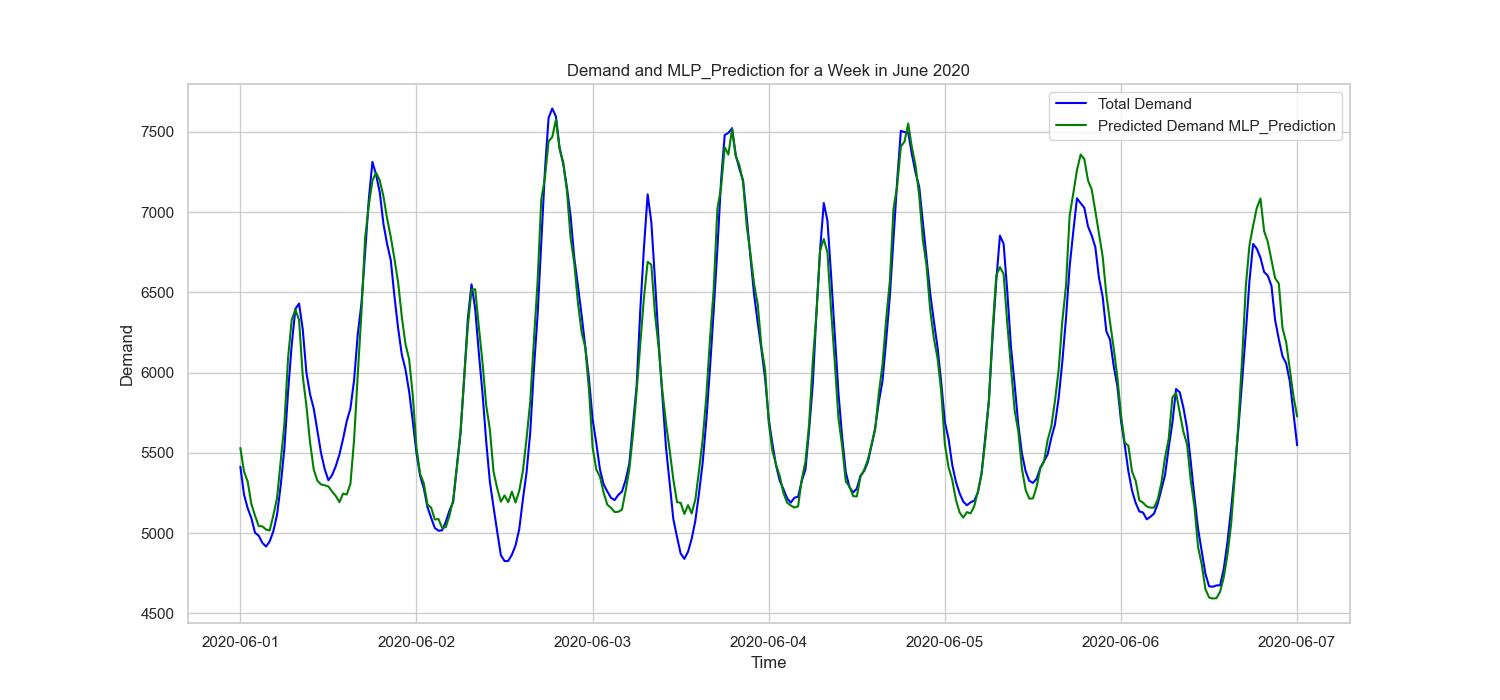
\includegraphics{img/mlp-prediction_june_2020.jpg}
\caption{MLP In June:}
\end{figure}

\begin{figure}
\centering
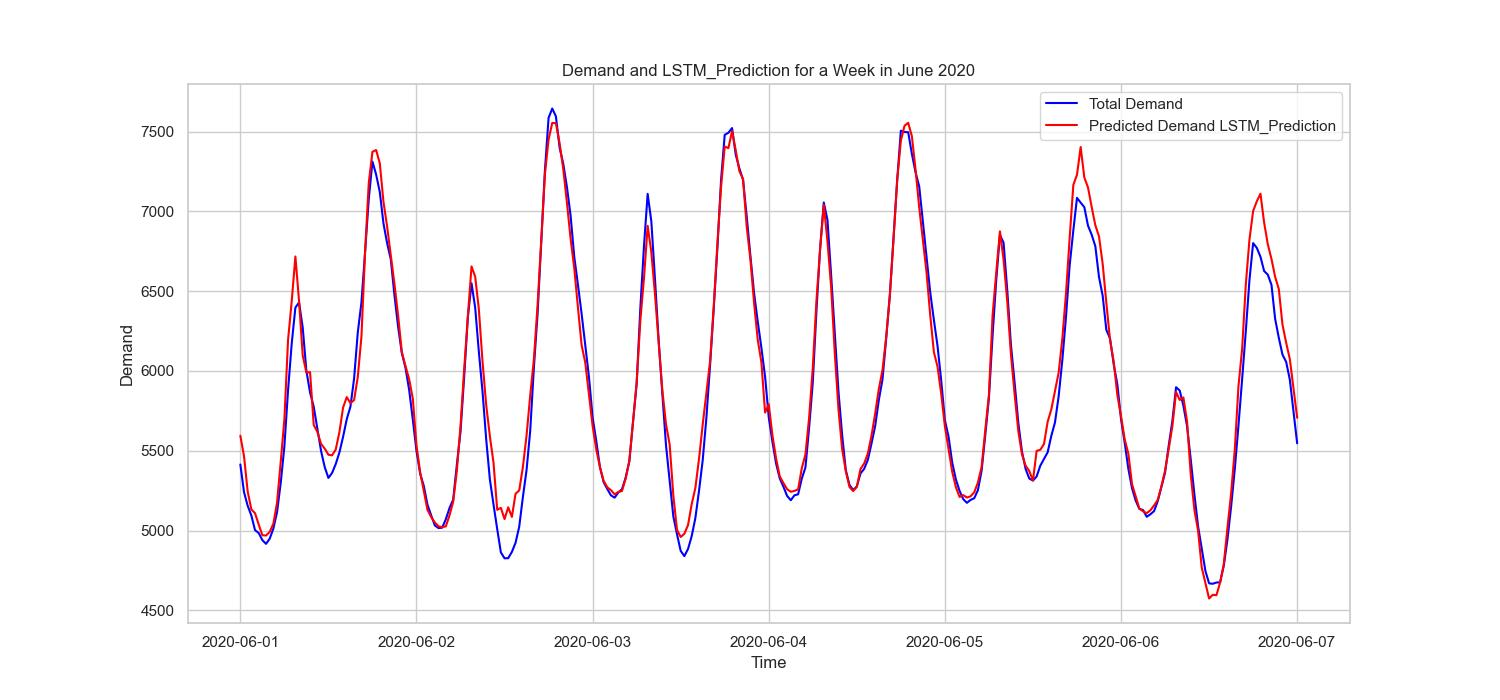
\includegraphics{img/lstm-prediction_june_2020.jpg}
\caption{LSTM In June:}
\end{figure}

\begin{figure}
\centering
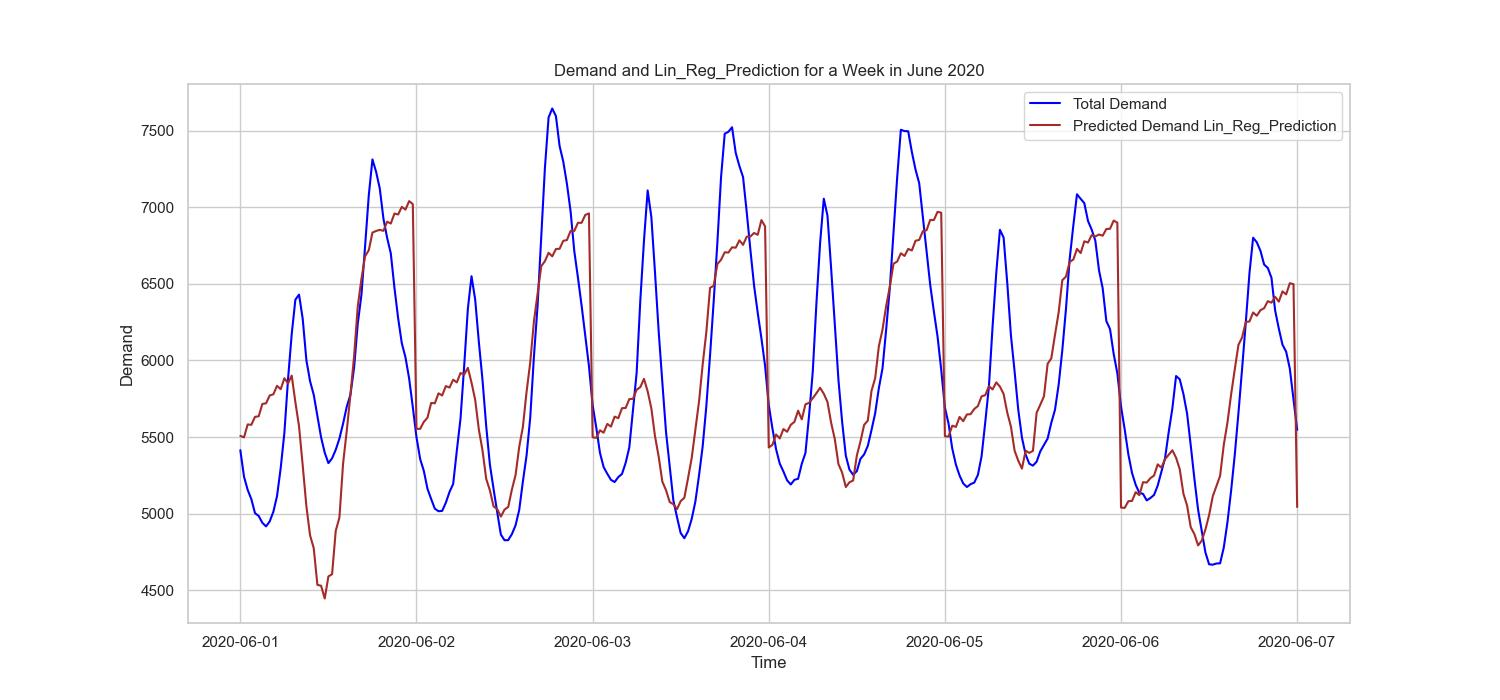
\includegraphics{img/lin-reg-prediction_june_2020.jpg}
\caption{Lin Reg Model in June:}
\end{figure}

\begin{figure}
\centering
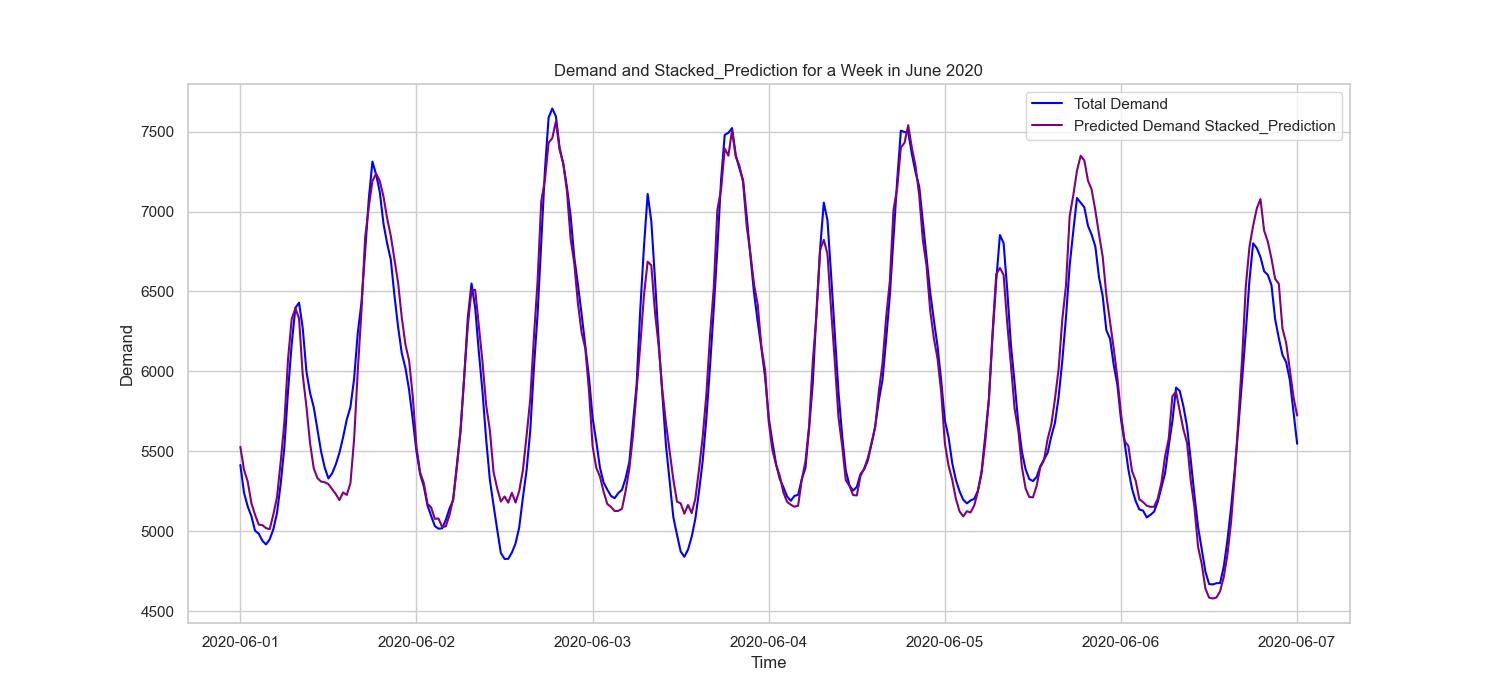
\includegraphics{img/stacked-prediction_june_2020.jpg}
\caption{Stacked Model In June:}
\end{figure}

\section{Discussion}\label{discussion}

From the data analysis above, we can see that there are some interesting
insights. From the results, it demonstrated that the prediction is more
accurate when we included rooftop solar panel power production into the
dataset. This is true for all states that we analyzed, (Victoria, South
Australia, and Queensland). That being said, the accuracy of the
prediction varies from state to state. The Queensland model that was
used for proof of concept showed a high R-squared value and low error
with or without solar power as one of the engineered features. The
R-squared value for LSTM model with solar feature and without is 0.9739
and 0.9662 respectively. The LSTM model with solar feature has a
slightly higher R-squared value but this still shows that both models
have a very high accuracy. Looking at other modeling techniques, all
models with solar features outperformed the models without, in terms of
r-squared value and error. Again, proofing the alternative hypothesis is
correct.

The same behavior can be observed on other states as well. The modeling
on Victoria and South Australia also shows better results by
implementing solar power production into the model. R-squared value for
Victoria model with and without solar power production are 0.9067 and
0.9033 respectively. Moreover, the solar model also has a lower error
when compared. However, the improvement is marginal when compared to the
improvement shown on the Queensland model. South Australia also showed
an R-square value improvement of 0.0578 when compared and an improvement
on RMSE and MAE, but it is worth noting that the R-squared value for
both models on South Australia is low when compared to Queensland and
Victoria. The best R-squared value for South Australia model is only at
0.7818 which is not sufficient for commercial demand forecasting. It is
possible that more features are required in order to make the model more
accurate. South Australia has a much lower population when compared to
Queensland and Victoria and hence has a lower demand, further research
will need to be conducted to find the cause.

\section{Conclusion and Further
Issues}\label{conclusion-and-further-issues}

As we conclude our study, we observe that the incorporation of
engineered features, particularly those related to solar data, has
markedly improved the predictive performance of all evaluated models.
The enhanced models have shown a significant increase in accuracy across
all key metrics, including MSE, RMSE, MAE, and the coefficient of
determination (\(R^2\)).

To further refine the predictive capabilities, we suggest the following
potential new engineered data features:

\begin{enumerate}
\def\labelenumi{\arabic{enumi}.}
\tightlist
\item
  \textbf{Behavioral Adjustments}: Incorporating data on school holidays
  and other public events that typically see a shift in electricity
  usage patterns.
\item
  \textbf{Household Efficiency Metrics}: Integrating data on energy
  efficiency improvements within households, such as the adoption of
  energy-efficient appliances and systems.
\item
  \textbf{Population Growth Projections}: Utilising demographic and
  urban planning data to adjust forecasts according to expected changes
  in population density and growth.
\item
  \textbf{Electric Vehicle Uptake}: Factoring in the increase in
  electric vehicle (EV) usage, which significantly impacts electricity
  demand due to charging requirements.
\end{enumerate}

For future analysis, several avenues could be explored:

\begin{enumerate}
\def\labelenumi{\arabic{enumi}.}
\tightlist
\item
  \textbf{Expansion of Feature Set}: Investigating additional
  environmental, economic, and behavioral factors in addition to the
  above that could further refine the predictive models.
\item
  \textbf{Longer Time Frame}: Extending the analysis to include a
  broader range of data over more recent years to validate the models
  against more varied conditions.
\item
  \textbf{Real-Time Analysis}: Developing a framework for real-time data
  analysis to enable dynamic forecasting that can adapt to rapid changes
  in demand patterns.
\end{enumerate}

These initiatives could provide deeper insights and drive the evolution
of forecasting methodologies to meet the complex demands of modern
energy management systems.

\section*{References}\label{references}
\addcontentsline{toc}{section}{References}

\phantomsection\label{refs}
\begin{CSLReferences}{0}{1}
\bibitem[\citeproctext]{ref-Abumohsen_Owda_Owda_2023}
Abumohsen, M., Owda, A.Y. and Owda, M. (2023) {`Electrical load
forecasting using LSTM, GRU, and RNN algorithms'}. \emph{Energies}
16(5), p. 2283. doi:
\href{https://doi.org/10.3390/en16052283}{10.3390/en16052283}.

\bibitem[\citeproctext]{ref-Amarasinghe_Marino_Manic_2017}
Amarasinghe, K., Marino, D.L. and Manic, M. (2017) {`Deep neural
networks for energy load forecasting'}. \emph{2017 IEEE 26th
International Symposium on Industrial Electronics (ISIE)}. doi:
\href{https://doi.org/10.1109/isie.2017.8001465}{10.1109/isie.2017.8001465}.

\bibitem[\citeproctext]{ref-Chung2014}
Chung, J., Gulcehre, C., Cho, K. and Bengio, Y. (2014) {`Empirical
evaluation of gated recurrent neural networks on sequence modeling'}.
\emph{arXiv preprint arXiv:1412.3555}

\bibitem[\citeproctext]{ref-Chung_Jang_2022}
Chung, J. and Jang, B. (2022) {`Accurate prediction of electricity
consumption using a hybrid CNN-LSTM model based on multivariable data'}.
\emph{PLOS ONE} 17(11). doi:
\href{https://doi.org/10.1371/journal.pone.0278071}{10.1371/journal.pone.0278071}.

\bibitem[\citeproctext]{ref-Hochreiter1997}
Hochreiter, S. and Schmidhuber, J. (1997) {`Long short-term memory'}.
\emph{Neural Computation} 9(8), pp. 1735--1780.

\bibitem[\citeproctext]{ref-Kang_Lim_Tayara_Chong_2020}
Kang, T., Lim, D.Y., Tayara, H. and Chong, K.T. (2020) {`Forecasting of
power demands using deep learning'}. \emph{Applied Sciences} 10(20), p.
7241. doi:
\href{https://doi.org/10.3390/app10207241}{10.3390/app10207241}.

\bibitem[\citeproctext]{ref-Kim_Cho_2019}
Kim, T.-Y. and Cho, S.-B. (2019) {`Predicting residential energy
consumption using CNN-LSTM neural networks'}. \emph{Energy} 182, pp.
72--81. doi:
\href{https://doi.org/10.1016/j.energy.2019.05.230}{10.1016/j.energy.2019.05.230}.

\bibitem[\citeproctext]{ref-Nielsen2015}
Nielsen, M. (2015) \emph{Neural networks and deep learning}.
Determination Press. Available at:
\url{http://neuralnetworksanddeeplearning.com/}.

\bibitem[\citeproctext]{ref-Torres_Martuxednez-uxc1lvarez_Troncoso_2022}
Torres, J.F., Martínez-Álvarez, F. and Troncoso, A. (2022) {`A DEEP LSTM
network for the spanish electricity consumption forecasting'}.
\emph{Neural Computing and Applications} 34(13), pp. 10533--10545. doi:
\href{https://doi.org/10.1007/s00521-021-06773-2}{10.1007/s00521-021-06773-2}.

\bibitem[\citeproctext]{ref-Wolpert1992}
Wolpert, D.H. (1992) {`Stacked generalization'}. \emph{Neural Networks}
5, pp. 241--259. doi:
\href{https://doi.org/10.1016/S0893-6080(05)80023-1}{10.1016/S0893-6080(05)80023-1}.

\bibitem[\citeproctext]{ref-Huang2016}
Yuansheng, H., Shenhai, H. and Jiayin, S. (2016) {`A novel hybrid method
for short-term power load forecasting'}. \emph{Journal of Electrical and
Computer Engineering} 2016, pp. 1--10. doi:
\href{https://doi.org/10.1155/2016/2165324}{10.1155/2016/2165324}.

\end{CSLReferences}

\bibliographystyle{elsarticle-harv}
\bibliography{references}

\section*{Appendix}\label{appendix}
\addcontentsline{toc}{section}{Appendix}

\subsection*{\texorpdfstring{\textbf{Codes}}{Codes}}\label{codes}
\addcontentsline{toc}{subsection}{\textbf{Codes}}

Add you codes here.

\subsection*{\texorpdfstring{\textbf{Tables}}{Tables}}\label{tables}
\addcontentsline{toc}{subsection}{\textbf{Tables}}

\end{document}
